% Options for packages loaded elsewhere
\PassOptionsToPackage{unicode}{hyperref}
\PassOptionsToPackage{hyphens}{url}
\PassOptionsToPackage{dvipsnames,svgnames,x11names}{xcolor}
%
\documentclass[
  letterpaper,
  DIV=11,
  numbers=noendperiod]{scrreprt}

\usepackage{amsmath,amssymb}
\usepackage{iftex}
\ifPDFTeX
  \usepackage[T1]{fontenc}
  \usepackage[utf8]{inputenc}
  \usepackage{textcomp} % provide euro and other symbols
\else % if luatex or xetex
  \usepackage{unicode-math}
  \defaultfontfeatures{Scale=MatchLowercase}
  \defaultfontfeatures[\rmfamily]{Ligatures=TeX,Scale=1}
\fi
\usepackage{lmodern}
\ifPDFTeX\else  
    % xetex/luatex font selection
\fi
% Use upquote if available, for straight quotes in verbatim environments
\IfFileExists{upquote.sty}{\usepackage{upquote}}{}
\IfFileExists{microtype.sty}{% use microtype if available
  \usepackage[]{microtype}
  \UseMicrotypeSet[protrusion]{basicmath} % disable protrusion for tt fonts
}{}
\makeatletter
\@ifundefined{KOMAClassName}{% if non-KOMA class
  \IfFileExists{parskip.sty}{%
    \usepackage{parskip}
  }{% else
    \setlength{\parindent}{0pt}
    \setlength{\parskip}{6pt plus 2pt minus 1pt}}
}{% if KOMA class
  \KOMAoptions{parskip=half}}
\makeatother
\usepackage{xcolor}
\setlength{\emergencystretch}{3em} % prevent overfull lines
\setcounter{secnumdepth}{5}
% Make \paragraph and \subparagraph free-standing
\ifx\paragraph\undefined\else
  \let\oldparagraph\paragraph
  \renewcommand{\paragraph}[1]{\oldparagraph{#1}\mbox{}}
\fi
\ifx\subparagraph\undefined\else
  \let\oldsubparagraph\subparagraph
  \renewcommand{\subparagraph}[1]{\oldsubparagraph{#1}\mbox{}}
\fi

\usepackage{color}
\usepackage{fancyvrb}
\newcommand{\VerbBar}{|}
\newcommand{\VERB}{\Verb[commandchars=\\\{\}]}
\DefineVerbatimEnvironment{Highlighting}{Verbatim}{commandchars=\\\{\}}
% Add ',fontsize=\small' for more characters per line
\usepackage{framed}
\definecolor{shadecolor}{RGB}{241,243,245}
\newenvironment{Shaded}{\begin{snugshade}}{\end{snugshade}}
\newcommand{\AlertTok}[1]{\textcolor[rgb]{0.68,0.00,0.00}{#1}}
\newcommand{\AnnotationTok}[1]{\textcolor[rgb]{0.37,0.37,0.37}{#1}}
\newcommand{\AttributeTok}[1]{\textcolor[rgb]{0.40,0.45,0.13}{#1}}
\newcommand{\BaseNTok}[1]{\textcolor[rgb]{0.68,0.00,0.00}{#1}}
\newcommand{\BuiltInTok}[1]{\textcolor[rgb]{0.00,0.23,0.31}{#1}}
\newcommand{\CharTok}[1]{\textcolor[rgb]{0.13,0.47,0.30}{#1}}
\newcommand{\CommentTok}[1]{\textcolor[rgb]{0.37,0.37,0.37}{#1}}
\newcommand{\CommentVarTok}[1]{\textcolor[rgb]{0.37,0.37,0.37}{\textit{#1}}}
\newcommand{\ConstantTok}[1]{\textcolor[rgb]{0.56,0.35,0.01}{#1}}
\newcommand{\ControlFlowTok}[1]{\textcolor[rgb]{0.00,0.23,0.31}{#1}}
\newcommand{\DataTypeTok}[1]{\textcolor[rgb]{0.68,0.00,0.00}{#1}}
\newcommand{\DecValTok}[1]{\textcolor[rgb]{0.68,0.00,0.00}{#1}}
\newcommand{\DocumentationTok}[1]{\textcolor[rgb]{0.37,0.37,0.37}{\textit{#1}}}
\newcommand{\ErrorTok}[1]{\textcolor[rgb]{0.68,0.00,0.00}{#1}}
\newcommand{\ExtensionTok}[1]{\textcolor[rgb]{0.00,0.23,0.31}{#1}}
\newcommand{\FloatTok}[1]{\textcolor[rgb]{0.68,0.00,0.00}{#1}}
\newcommand{\FunctionTok}[1]{\textcolor[rgb]{0.28,0.35,0.67}{#1}}
\newcommand{\ImportTok}[1]{\textcolor[rgb]{0.00,0.46,0.62}{#1}}
\newcommand{\InformationTok}[1]{\textcolor[rgb]{0.37,0.37,0.37}{#1}}
\newcommand{\KeywordTok}[1]{\textcolor[rgb]{0.00,0.23,0.31}{#1}}
\newcommand{\NormalTok}[1]{\textcolor[rgb]{0.00,0.23,0.31}{#1}}
\newcommand{\OperatorTok}[1]{\textcolor[rgb]{0.37,0.37,0.37}{#1}}
\newcommand{\OtherTok}[1]{\textcolor[rgb]{0.00,0.23,0.31}{#1}}
\newcommand{\PreprocessorTok}[1]{\textcolor[rgb]{0.68,0.00,0.00}{#1}}
\newcommand{\RegionMarkerTok}[1]{\textcolor[rgb]{0.00,0.23,0.31}{#1}}
\newcommand{\SpecialCharTok}[1]{\textcolor[rgb]{0.37,0.37,0.37}{#1}}
\newcommand{\SpecialStringTok}[1]{\textcolor[rgb]{0.13,0.47,0.30}{#1}}
\newcommand{\StringTok}[1]{\textcolor[rgb]{0.13,0.47,0.30}{#1}}
\newcommand{\VariableTok}[1]{\textcolor[rgb]{0.07,0.07,0.07}{#1}}
\newcommand{\VerbatimStringTok}[1]{\textcolor[rgb]{0.13,0.47,0.30}{#1}}
\newcommand{\WarningTok}[1]{\textcolor[rgb]{0.37,0.37,0.37}{\textit{#1}}}

\providecommand{\tightlist}{%
  \setlength{\itemsep}{0pt}\setlength{\parskip}{0pt}}\usepackage{longtable,booktabs,array}
\usepackage{calc} % for calculating minipage widths
% Correct order of tables after \paragraph or \subparagraph
\usepackage{etoolbox}
\makeatletter
\patchcmd\longtable{\par}{\if@noskipsec\mbox{}\fi\par}{}{}
\makeatother
% Allow footnotes in longtable head/foot
\IfFileExists{footnotehyper.sty}{\usepackage{footnotehyper}}{\usepackage{footnote}}
\makesavenoteenv{longtable}
\usepackage{graphicx}
\makeatletter
\def\maxwidth{\ifdim\Gin@nat@width>\linewidth\linewidth\else\Gin@nat@width\fi}
\def\maxheight{\ifdim\Gin@nat@height>\textheight\textheight\else\Gin@nat@height\fi}
\makeatother
% Scale images if necessary, so that they will not overflow the page
% margins by default, and it is still possible to overwrite the defaults
% using explicit options in \includegraphics[width, height, ...]{}
\setkeys{Gin}{width=\maxwidth,height=\maxheight,keepaspectratio}
% Set default figure placement to htbp
\makeatletter
\def\fps@figure{htbp}
\makeatother

\KOMAoption{captions}{tableheading}
\makeatletter
\makeatother
\makeatletter
\@ifpackageloaded{bookmark}{}{\usepackage{bookmark}}
\makeatother
\makeatletter
\@ifpackageloaded{caption}{}{\usepackage{caption}}
\AtBeginDocument{%
\ifdefined\contentsname
  \renewcommand*\contentsname{Table of contents}
\else
  \newcommand\contentsname{Table of contents}
\fi
\ifdefined\listfigurename
  \renewcommand*\listfigurename{List of Figures}
\else
  \newcommand\listfigurename{List of Figures}
\fi
\ifdefined\listtablename
  \renewcommand*\listtablename{List of Tables}
\else
  \newcommand\listtablename{List of Tables}
\fi
\ifdefined\figurename
  \renewcommand*\figurename{Figure}
\else
  \newcommand\figurename{Figure}
\fi
\ifdefined\tablename
  \renewcommand*\tablename{Table}
\else
  \newcommand\tablename{Table}
\fi
}
\@ifpackageloaded{float}{}{\usepackage{float}}
\floatstyle{ruled}
\@ifundefined{c@chapter}{\newfloat{codelisting}{h}{lop}}{\newfloat{codelisting}{h}{lop}[chapter]}
\floatname{codelisting}{Listing}
\newcommand*\listoflistings{\listof{codelisting}{List of Listings}}
\makeatother
\makeatletter
\@ifpackageloaded{caption}{}{\usepackage{caption}}
\@ifpackageloaded{subcaption}{}{\usepackage{subcaption}}
\makeatother
\makeatletter
\@ifpackageloaded{tcolorbox}{}{\usepackage[skins,breakable]{tcolorbox}}
\makeatother
\makeatletter
\@ifundefined{shadecolor}{\definecolor{shadecolor}{rgb}{.97, .97, .97}}
\makeatother
\makeatletter
\makeatother
\makeatletter
\makeatother
\makeatletter
\@ifpackageloaded{tikz}{}{\usepackage{tikz}}
\makeatother
        \newcommand*\circled[1]{\tikz[baseline=(char.base)]{
          \node[shape=circle,draw,inner sep=1pt] (char) {{\scriptsize#1}};}}  
                  
\ifLuaTeX
  \usepackage{selnolig}  % disable illegal ligatures
\fi
\IfFileExists{bookmark.sty}{\usepackage{bookmark}}{\usepackage{hyperref}}
\IfFileExists{xurl.sty}{\usepackage{xurl}}{} % add URL line breaks if available
\urlstyle{same} % disable monospaced font for URLs
\hypersetup{
  pdftitle={R语言快速入门},
  pdfauthor={Shalom},
  colorlinks=true,
  linkcolor={blue},
  filecolor={Maroon},
  citecolor={Blue},
  urlcolor={Blue},
  pdfcreator={LaTeX via pandoc}}

\title{R语言快速入门}
\author{Shalom}
\date{2023-08-13}

\begin{document}
\maketitle
\ifdefined\Shaded\renewenvironment{Shaded}{\begin{tcolorbox}[breakable, sharp corners, boxrule=0pt, enhanced, borderline west={3pt}{0pt}{shadecolor}, interior hidden, frame hidden]}{\end{tcolorbox}}\fi

\renewcommand*\contentsname{Table of contents}
{
\hypersetup{linkcolor=}
\setcounter{tocdepth}{2}
\tableofcontents
}
\bookmarksetup{startatroot}

\hypertarget{ux524dux8a00}{%
\chapter*{前言}\label{ux524dux8a00}}
\addcontentsline{toc}{chapter}{前言}

\markboth{前言}{前言}

这是一本只讲干货的R语言入门书籍,希望对您有所帮助.

\hypertarget{rux80fdux505aux4ec0ux4e48}{%
\section*{R能做什么?}\label{rux80fdux505aux4ec0ux4e48}}
\addcontentsline{toc}{section}{R能做什么?}

\markright{R能做什么?}

\begin{itemize}
\item
  数据分析
\item
  数据可视化 \href{https://rrr.is/covid}{上海新冠}
  \href{https://chart.rlearner.com}{R作图}
\item
  爬取数据 \href{https://blog.rlearner.com/r/rvest-base.html}{爬数据}
\item
  写博客 \href{https://blog.rlearner.com}{Shalom的博客}
\item
  做网站 \href{https://shiny.posit.co/r/gallery/}{Shiny}
  \href{https://learn-r.shinyapps.io/epi-china/}{中华流病}
\item
  写书 \href{https://bookdown.org/}{bookdown}
\end{itemize}

\hypertarget{ux5982ux4f55ux5b66ux597drux8bedux8a00}{%
\section*{如何学好R语言?}\label{ux5982ux4f55ux5b66ux597drux8bedux8a00}}
\addcontentsline{toc}{section}{如何学好R语言?}

\markright{如何学好R语言?}

\begin{itemize}
\item
  \textbf{夯实基础}。欲速则不达,打好基础,后续学起来会很轻松。

  比如,你要懂得什么是数据框(dataframe),什么是行(row)和列(column),什么是观测(observation)和变量(variable),什么是包(package)和函数(function),什么是向量(vector)和列表(list),基本的术语不算多,掌握好基础你才能很好地组织你的问题,学会提问也是一门学问。初学者切忌啥都不懂,就一心只想实现某个功能,别的一概不问,这样的学习者注定学不好一门语言。
\item
  \textbf{博观约取}。多了解R能做什么,在遇到问题的时候才会想起来用什么。如果自己阅读过的话那就翻出来针对性地仔细阅读,如果是自己也没遇到过得问题,那么请用基本的数据科学术语描述你的问题(例如:如何给数据框增加一列新的变量),然后在互联网上或者交流社区提出你的问题,我相信,当你把你的问题表述清楚的时候,别人是很乐意回答你的问题的。学会正确的提问真的很重要!
\item
  \textbf{勤敲代码}。眼过千遍不如手敲一遍。刚开始写代码总是需要模仿或者参考别人的代码,当敲的多了,你自然会记住代码。学R的最好方式是实践,所有在Excel中的操作都能在R中实现,从一个简单的筛选做起,将你之前用EXCEL完成的工作换成用R来完成,每一次练习都会提升你的编程技能。
\end{itemize}

\hypertarget{rux8bedux8a00ux5b66ux4e60ux8d44ux6599}{%
\section*{R语言学习资料}\label{rux8bedux8a00ux5b66ux4e60ux8d44ux6599}}
\addcontentsline{toc}{section}{R语言学习资料}

\markright{R语言学习资料}

\begin{itemize}
\item
  \href{https://hub.rlearner.com}{hub.rlearner.com}
  该网站汇集了众多R学习资源
\item
  \href{https://rlearner.com}{R论坛} R学习交流社区
\item
  \href{https://blog.rlearner.com/r-index.html}{我的博客}
\item
  微信公众号:R数据分析与可视化

  \includegraphics{images/gzh-green.png}
\end{itemize}

\part{基础篇}

\hypertarget{ux5b89ux88c5}{%
\chapter{安装}\label{ux5b89ux88c5}}

安装R和RStudio是进行数据分析和统计建模的重要步骤。以下是在Windows操作系统上安装R和RStudio的简要步骤说明:

\hypertarget{ux5b89ux88c5r}{%
\section{安装R}\label{ux5b89ux88c5r}}

\begin{enumerate}
\def\labelenumi{\arabic{enumi}.}
\item
  \textbf{下载R安装程序:}
  访问\href{https://cran.r-project.org/mirrors.html}{R官方网站},选择一个离您位置较近的镜像站点,然后在页面上找到适合您操作系统的安装程序链接。
\item
  \textbf{运行安装程序:}
  下载完成后,运行下载的安装程序。您可能会看到一些安装选项,可以根据您的偏好进行选择,但通常情况下,您可以选择默认选项。
\item
  \textbf{选择安装位置:}
  在安装过程中,您可能需要选择R的安装位置。通常情况下,保留默认安装位置即可。
\item
  \textbf{完成安装:}
  完成上述步骤后,安装程序将开始将R安装到您的计算机上。等待安装完成。
\end{enumerate}

\hypertarget{ux5b89ux88c5rstudio}{%
\section{安装RStudio}\label{ux5b89ux88c5rstudio}}

\begin{enumerate}
\def\labelenumi{\arabic{enumi}.}
\item
  \textbf{下载RStudio安装程序:}
  访问\href{https://www.rstudio.com/products/rstudio/download/}{RStudio官方网站},找到免费版本的RStudio
  Desktop,并选择适合您操作系统的安装程序。
\item
  \textbf{运行安装程序:}
  下载完成后,运行安装程序。同样,您可能会看到一些安装选项,可以根据需要进行选择。
\item
  \textbf{完成安装:}
  安装程序将开始将RStudio安装到您的计算机上。等待安装完成。
\end{enumerate}

\hypertarget{ux542fux52a8rstudio}{%
\section{启动RStudio}\label{ux542fux52a8rstudio}}

安装完成后,您可以从开始菜单(在Windows上)或应用程序列表中找到RStudio的图标,双击它以启动RStudio。

请注意,这里提供的是Windows操作系统上的步骤。如果您使用的是Mac或Linux操作系统,步骤可能会稍有不同,但基本原理是相似的。安装完成后,您可以在RStudio中轻松编写和运行R代码,进行数据分析和统计建模等工作。

\hypertarget{rstudioux4e0erux7684ux533aux522bux4e0eux8054ux7cfb}{%
\chapter{Rstudio与R的区别与联系}\label{rstudioux4e0erux7684ux533aux522bux4e0eux8054ux7cfb}}

RStudio是一款用于编写和执行R代码的集成开发环境(IDE)。它可以帮助您管理工作空间、查看数据集和图形、执行代码并可视化结果等。
\#\# 安装与使用 下面是安装和使用RStudio的步骤:

\begin{enumerate}
\def\labelenumi{\arabic{enumi}.}
\item
  从RStudio的\href{https://posit.co/downloads/}{官方网站}下载最新版本的安装包。
\item
  双击安装包文件,并按照安装向导的提示完成安装。
\item
  安装完成后,打开RStudio,在左侧的控制台中输入R代码并执行。
\item
  在左上角的''文件''菜单中,可以打开或保存代码文件。
\item
  在右侧的''工作空间和环境''窗口中,可以查看当前工作空间中的对象和数据集。
\item
  在右侧的''图形''窗口中,可以查看图形和交互式图形。
\end{enumerate}

RStudio是一款用于编写和执行R代码的集成开发环境(IDE),它可以帮助您管理工作空间、查看数据集和图形、执行代码并可视化结果等。R是一种编程语言,用于数据分析和统计计算。

RStudio与R之间的关系可以理解为电脑和操作系统之间的关系,即RStudio是为R语言提供一个更友好的操作界面的工具。您可以使用RStudio进行R代码的编写和执行,也可以直接使用R语言进行编程。

总而言之,RStudio是R语言的一个友好的用户界面,通过它可以更轻松地使用R语言进行数据分析和统计计算。但RStudio本身并不是R语言,它仅仅是一个工具,需要依赖R语言

\hypertarget{rstudioux7684ux5e38ux7528ux5febux6377ux952eux6709ux54eaux4e9b}{%
\section{Rstudio的常用快捷键有哪些?}\label{rstudioux7684ux5e38ux7528ux5febux6377ux952eux6709ux54eaux4e9b}}

\begin{itemize}
\item
  执行R代码并跳到下一行:按\texttt{Ctrl\ +\ Enter}键可以快速执行当前光标所在行的R代码,并跳到下一行。
\item
  快速执行R代码:按\texttt{Alt\ +\ Enter}键可以快速执行当前光标所在行的R代码。
\item
  快速注释/取消注释:按\texttt{Ctrl\ +\ Shift\ +\ C}键可以快速将当前光标所在行的R代码注释掉,再次按下该快捷键可以取消注释。
\end{itemize}

\hypertarget{rstudioux65b0ux5efarux9879ux76eeproject}{%
\section{Rstudio新建R项目(Project)}\label{rstudioux65b0ux5efarux9879ux76eeproject}}

RStudio提供了一个项目管理功能,可以帮助您管理项目代码。下面是使用RStudio新建项目代码的步骤:

\begin{enumerate}
\def\labelenumi{\arabic{enumi}.}
\item
  打开RStudio,在''文件''菜单中,选择''新建项目''。
\item
  在弹出的对话框中,选择项目的存储位置和类型。
\item
  点击''确定''按钮,RStudio就会为您创建一个新项目。
\item
  在项目中,您可以通过''文件''菜单或''文件浏览器''窗口来创建、打开、保存和关闭R代码文件。
\item
  在项目中,您可以通过''代码''菜单或''编辑''按钮来编辑R代码文件。
\item
  在项目中,您可以通过''控制台''窗口来输入和执行R代码。
\item
  在项目中,您可以通过''终端''窗口来执行Shell命令。
\item
  在项目中,您可以通过''工作空间和环境''窗口来查看当前工作空间中的对象和数据集。
\end{enumerate}

\hypertarget{rux9879ux76eeux7684ux4e00ux822cux6587ux4ef6ux6784ux6210}{%
\section{R项目的一般文件构成}\label{rux9879ux76eeux7684ux4e00ux822cux6587ux4ef6ux6784ux6210}}

RStudio
project项目是一种用于管理R代码和数据的文件夹,通常包含以下文件和文件夹:

\begin{itemize}
\tightlist
\item
  .Rproj文件:这是项目的主文件,RStudio会识别它并打开项目。
\item
  .Rhistory文件:这是项目的历史记录文件,包含执行的所有R代码。
\item
  .RData文件:这是项目的工作空间文件,包含执行的所有R代码中定义的对象和数据集。
\item
  .Renviron文件:这是项目的环境变量文件,包含定义的所有环境变量。
\item
  data文件夹:这是项目的数据文件夹,包含项目中使用的所有数据文件。
\item
  R文件夹:这是项目的代码文件夹,包含项目中使用的所有R代码文件。
\end{itemize}

\hypertarget{ux57faux672cux6570ux636eux7c7bux578b}{%
\chapter{基本数据类型}\label{ux57faux672cux6570ux636eux7c7bux578b}}

R语言有多种基本的数据类型,包括整型数据(integer)、浮点型数据(floating
point)、字符型数据(character)、布尔型数据(logical)、复数型数据(complex)和因子类型数据(factor)。

\begin{itemize}
\tightlist
\item
  整型数据: 表示整数值,例如 \texttt{1} 或 \texttt{-4}。
\item
  浮点型数据: 表示带小数点的数值,例如 \texttt{3.14} 或 \texttt{-0.12}。
\item
  字符型数据: 表示文本字符串,例如 \texttt{"hello"} 或
  \texttt{"R\ is\ a\ programming\ language"}。
\item
  布尔型数据: 表示布尔值,即逻辑值,只有两个值,即 \texttt{TRUE} 或
  \texttt{FALSE}。
\item
  复数型数据: 表示复数,例如 \texttt{3\ +\ 2i} 或 \texttt{-1\ +\ 4i}。
\item
  因子类型数据: 用于表示分类变量,例如性别 (男、女) 或季节
  (春、夏、秋、冬)。
\end{itemize}

\hypertarget{ux6570ux636eux7ed3ux6784ux7c7bux578b}{%
\section{数据结构类型}\label{ux6570ux636eux7ed3ux6784ux7c7bux578b}}

R语言中有多种数据结构类型,这些类型都有各自的名称和意义。下面是一些常见的数据结构类型:

\begin{enumerate}
\def\labelenumi{\arabic{enumi}.}
\item
  向量(vector):这种类型的数据是一个一维的数值序列,例如c(1, 2, 3,
  4)。
\item
  矩阵(matrix):这种类型的数据是一个二维的数值表格,例如matrix(1:9,
  nrow = 3)。
\item
  数组(array):这种类型的数据是一个多维的数值表格,例如array(1:8, dim
  = c(2, 2, 2))。
\item
  数据框(data.frame):这种类型的数据是一个二维的表格,可以包含不同类型的变量,例如data.frame(x
  = 1:3, y = c(``a'', ``b'', ``c''))。
\item
  列表(list):这种类型的数据是一个有序的元素集合,可以包含不同类型的对象,例如list(1,
  ``hello'', TRUE)。
\end{enumerate}

\hypertarget{ux6570ux636eux6846dataframeux7684ux5e38ux89c1ux64cdux4f5c}{%
\section{数据框(dataframe)的常见操作}\label{ux6570ux636eux6846dataframeux7684ux5e38ux89c1ux64cdux4f5c}}

数据框是 R
语言中一种常用的数据结构,它是一个二维数据表,用于存储一组不同类型的数据,每列数据都有一个对应的列名。

一些常见的数据框操作包括:

\begin{itemize}
\tightlist
\item
  创建数据框: 使用 \texttt{data.frame()} 函数创建数据框。
\item
  查看数据框: 使用 \texttt{head()} 和 \texttt{tail()}
  函数查看数据框的前几行和后几行,使用 \texttt{str()}
  函数查看数据框的数据类型和结构。
\item
  选择数据框中的某一列: 使用 \texttt{\$} 操作符选择某一列。
\item
  选择数据框中的某一行: 使用行索引选择某一行。
\item
  选择数据框中的某一个值: 使用行索引和列名选择某一个值。
\item
  添加数据框列: 使用 \texttt{\$} 操作符添加新的列。
\item
  添加数据框行: 使用 \texttt{rbind()} 函数添加新的行。
\item
  删除数据框列: 使用 \texttt{\$} 操作符删除某一列。
\item
  删除数据框行: 使用行索引删除某一行。
\item
  排序数据框: 使用 \texttt{order()} 函数对某一列或多列进行排序。
\item
  过滤数据框: 使用布尔运算符过滤数据框中符合条件的行。
\end{itemize}

\hypertarget{ux4ee3ux7801ux793aux4f8b}{%
\section{代码示例}\label{ux4ee3ux7801ux793aux4f8b}}

\begin{Shaded}
\begin{Highlighting}[]
\CommentTok{\# 创建一个数据框}
\NormalTok{my\_data\_frame }\OtherTok{\textless{}{-}} \FunctionTok{data.frame}\NormalTok{(}
  \AttributeTok{id =} \FunctionTok{c}\NormalTok{(}\DecValTok{1}\NormalTok{, }\DecValTok{2}\NormalTok{, }\DecValTok{3}\NormalTok{),}
  \AttributeTok{name =} \FunctionTok{c}\NormalTok{(}\StringTok{"Alice"}\NormalTok{, }\StringTok{"Bob"}\NormalTok{, }\StringTok{"Charlie"}\NormalTok{),}
  \AttributeTok{age =} \FunctionTok{c}\NormalTok{(}\DecValTok{20}\NormalTok{, }\DecValTok{25}\NormalTok{, }\DecValTok{30}\NormalTok{),}
  \AttributeTok{gender =} \FunctionTok{c}\NormalTok{(}\StringTok{"F"}\NormalTok{, }\StringTok{"M"}\NormalTok{, }\StringTok{"M"}\NormalTok{)}
\NormalTok{)}

\CommentTok{\# 查看数据框的前几行}
\FunctionTok{head}\NormalTok{(my\_data\_frame)}
\end{Highlighting}
\end{Shaded}

\begin{verbatim}
  id    name age gender
1  1   Alice  20      F
2  2     Bob  25      M
3  3 Charlie  30      M
\end{verbatim}

\begin{Shaded}
\begin{Highlighting}[]
\CommentTok{\# 查看数据框的后几行}
\FunctionTok{tail}\NormalTok{(my\_data\_frame)}
\end{Highlighting}
\end{Shaded}

\begin{verbatim}
  id    name age gender
1  1   Alice  20      F
2  2     Bob  25      M
3  3 Charlie  30      M
\end{verbatim}

\begin{Shaded}
\begin{Highlighting}[]
\CommentTok{\# 查看数据框的数据类型和结构}
\FunctionTok{str}\NormalTok{(my\_data\_frame)}
\end{Highlighting}
\end{Shaded}

\begin{verbatim}
'data.frame':   3 obs. of  4 variables:
 $ id    : num  1 2 3
 $ name  : chr  "Alice" "Bob" "Charlie"
 $ age   : num  20 25 30
 $ gender: chr  "F" "M" "M"
\end{verbatim}

\begin{Shaded}
\begin{Highlighting}[]
\CommentTok{\# 选择数据框中的某一列}
\NormalTok{my\_data\_frame}\SpecialCharTok{$}\NormalTok{name}
\end{Highlighting}
\end{Shaded}

\begin{verbatim}
[1] "Alice"   "Bob"     "Charlie"
\end{verbatim}

\begin{Shaded}
\begin{Highlighting}[]
\CommentTok{\# 选择数据框中的某一行}
\NormalTok{my\_data\_frame[}\DecValTok{2}\NormalTok{, ]}
\end{Highlighting}
\end{Shaded}

\begin{verbatim}
  id name age gender
2  2  Bob  25      M
\end{verbatim}

\begin{Shaded}
\begin{Highlighting}[]
\CommentTok{\# 选择数据框中的某一个值}
\NormalTok{my\_data\_frame[}\DecValTok{2}\NormalTok{, }\StringTok{"name"}\NormalTok{]}
\end{Highlighting}
\end{Shaded}

\begin{verbatim}
[1] "Bob"
\end{verbatim}

\begin{Shaded}
\begin{Highlighting}[]
\CommentTok{\# 添加数据框列}
\NormalTok{my\_data\_frame}\SpecialCharTok{$}\NormalTok{score }\OtherTok{\textless{}{-}} \FunctionTok{c}\NormalTok{(}\DecValTok{90}\NormalTok{, }\DecValTok{85}\NormalTok{, }\DecValTok{80}\NormalTok{)}

\CommentTok{\# 添加数据框行}
\NormalTok{new\_row }\OtherTok{\textless{}{-}} \FunctionTok{data.frame}\NormalTok{(}\AttributeTok{id =} \DecValTok{4}\NormalTok{, }\AttributeTok{name =} \StringTok{"David"}\NormalTok{, }\AttributeTok{age =} \DecValTok{32}\NormalTok{, }\AttributeTok{gender =} \StringTok{"M"}\NormalTok{, }\AttributeTok{score =} \DecValTok{75}\NormalTok{)}
\NormalTok{my\_data\_frame }\OtherTok{\textless{}{-}} \FunctionTok{rbind}\NormalTok{(my\_data\_frame, new\_row)}

\CommentTok{\# 删除数据框列}
\NormalTok{my\_data\_frame}\SpecialCharTok{$}\NormalTok{score }\OtherTok{\textless{}{-}} \ConstantTok{NULL}

\CommentTok{\# 删除数据框行}
\NormalTok{my\_data\_frame }\OtherTok{\textless{}{-}}\NormalTok{ my\_data\_frame[}\SpecialCharTok{{-}}\DecValTok{2}\NormalTok{, ]}

\CommentTok{\# 排序数据框}
\NormalTok{my\_data\_frame }\OtherTok{\textless{}{-}}\NormalTok{ my\_data\_frame[}\FunctionTok{order}\NormalTok{(my\_data\_frame}\SpecialCharTok{$}\NormalTok{age), ]}

\CommentTok{\# 过滤数据框}
\NormalTok{my\_data\_frame[my\_data\_frame}\SpecialCharTok{$}\NormalTok{age }\SpecialCharTok{\textgreater{}=} \DecValTok{25}\NormalTok{, ]}
\end{Highlighting}
\end{Shaded}

\begin{verbatim}
  id    name age gender
3  3 Charlie  30      M
4  4   David  32      M
\end{verbatim}

\hypertarget{ux884cux7d22ux5f15ux548cux5217ux7d22ux5f15}{%
\section{行索引和列索引}\label{ux884cux7d22ux5f15ux548cux5217ux7d22ux5f15}}

在 R
语言中,数据框是一种二维数据表,其中每行表示一个观察值,每列表示一个变量。数据框的行索引和列索引是用来确定某一个特定的数据值的位置的方法。

\begin{itemize}
\tightlist
\item
  行索引: 数据框的行索引是从 1
  开始的正整数,用来标识每一行。例如,在上面的代码中,第一行的行索引是
  1,第二行的行索引是 2,以此类推。
\item
  列索引:
  数据框的列索引是列名,用来标识每一列。例如,在上面的代码中,第一列的列索引是
  \texttt{id},第二列的列索引是 \texttt{name},以此类推。
\end{itemize}

我们可以使用行索引和列索引来选择数据框中的某一个值。例如,如果我们想选择第二行第三列的值,可以使用
\texttt{my\_data\_frame{[}2,\ "age"{]}} 这样的语法。

\hypertarget{ux884cux7d22ux5f15ux548cux5217ux7d22ux5f15ux7684ux5e38ux89c1ux7528ux6cd5}{%
\section{行索引和列索引的常见用法}\label{ux884cux7d22ux5f15ux548cux5217ux7d22ux5f15ux7684ux5e38ux89c1ux7528ux6cd5}}

行索引和列索引在 R
语言中都非常常见,它们有许多用途。下面是一些常见的行索引和列索引的用法:

\begin{itemize}
\tightlist
\item
  选择数据框中的某一个值:
  可以使用行索引和列索引选择数据框中的某一个值。例如,\texttt{my\_data\_frame{[}2,\ "name"{]}}
  表示选择第二行第 \texttt{name} 列的值。
\item
  添加数据框行: 可以使用行索引和 \texttt{rbind()}
  函数添加新的行到数据框中。例如,\texttt{my\_data\_frame\ \textless{}-\ rbind(my\_data\_frame,\ new\_row)}
  表示将新的行 \texttt{new\_row} 添加到数据框 \texttt{my\_data\_frame}
  的末尾。
\item
  删除数据框行:
  可以使用行索引删除数据框中的某一行。例如,\texttt{my\_data\_frame\ \textless{}-\ my\_data\_frame{[}-2,\ {]}}
  表示删除数据框 \texttt{my\_data\_frame} 中的第二行。
\item
  排序数据框: 可以使用行索引和 \texttt{order()}
  函数对数据框进行排序。例如,\texttt{my\_data\_frame\ \textless{}-\ my\_data\_frame{[}order(my\_data\_frame\$age),\ {]}}
  表示根据 \texttt{age} 列对数据框 `
\end{itemize}

\hypertarget{ux5728rux8bedux8a00ux4e2dux7684ux542bux4e49}{%
\section{{[}{]}在R语言中的含义}\label{ux5728rux8bedux8a00ux4e2dux7684ux542bux4e49}}

在 R 语言中,\texttt{{[}{]}}
符号用来表示数据结构的索引。具体来说,它表示选择数据结构中的某一部分。例如,如果
\texttt{my\_data} 是一个数据框,那么 \texttt{my\_data{[}2,\ "name"{]}}
表示选择数据框 \texttt{my\_data} 中的第二行第 \texttt{name} 列的值。

在 R 语言中,\texttt{{[}{]}}
符号还可以用来进行其他操作,例如排序、过滤、删除等。它还可以用来创建新的数据结构,例如向量、数组、数据框等。有关具体用法,您可以参考
R 语言的相关文档和教程。

\hypertarget{rux8bedux8a00ux4e2d-ux548cux7684ux533aux522b}{%
\section{R语言中\textless-和=的区别}\label{rux8bedux8a00ux4e2d-ux548cux7684ux533aux522b}}

在 R 语言中,\texttt{\textless{}-} 和 \texttt{=}
都可以用来赋值,但它们之间还是有一些区别的。

\begin{itemize}
\tightlist
\item
  \texttt{\textless{}-}: 这是 R
  语言中最常用的赋值操作符。它用来将右侧的值赋给左侧的变量。例如,\texttt{x\ \textless{}-\ 5}
  表示将 5 赋给变量 \texttt{x}。
\item
  \texttt{=}: 这是 R 语言中次常用的赋值操作符。它的语法与
  \texttt{\textless{}-}
  类似,也用来将右侧的值赋给左侧的变量。例如,\texttt{x\ =\ 5} 也表示将
  5 赋给变量 \texttt{x}。
\end{itemize}

在实际使用中,\texttt{\textless{}-} 和 \texttt{=}
的区别主要在于语义上的差异。通常来说,\texttt{\textless{}-}
操作符更加符合人类的思维方式,因为它更加形象地表达了赋值的意义(即将值从右向左流动)。而
\texttt{=} 操作符则更像是一个等号,表示变量与值相等。

在 R 语言中,一般来说,\texttt{\textless{}-} 操作符更加常用,并且在 R
语言的文档和教程中也更常见。但 \texttt{=}
操作符也是可以使用的,它们之间并没有严格的限制。您可以根据个人喜好来选择使用哪一个。

总的来说,建议使用 \texttt{\textless{}-}
操作符进行赋值,这样能够更好地保持统一,并且能够更方便地理解代码。

\hypertarget{ux4e2dux7f3aux7701ux884cux7d22ux5f15ux548cux5217ux7d22ux5f15ux7684ux610fux4e49}{%
\section{{[}{]}中缺省行索引和列索引的意义}\label{ux4e2dux7f3aux7701ux884cux7d22ux5f15ux548cux5217ux7d22ux5f15ux7684ux610fux4e49}}

在 R 语言中,当 \texttt{{[}{]}}
符号中的行索引或列索引缺省时,它们会被自动填充为默认值。

对于行索引,如果缺省,默认值是 1:n,其中 n 是数据框中的行数。例如,如果
\texttt{my\_data} 是一个数据框,那么 \texttt{my\_data{[},\ "name"{]}} 和
\texttt{my\_data{[}1:n,\ "name"{]}} 是等价的,都表示选择数据框
\texttt{my\_data} 中的所有行的 \texttt{name} 列。

对于列索引,如果缺省,默认值是所有列的名称。例如,如果 \texttt{my\_data}
是一个数据框,那么 \texttt{my\_data{[}2,\ {]}} 和
\texttt{my\_data{[}2,\ colnames(my\_data){]}} 是等价的,都表示选择数据框
\texttt{my\_data} 中的第二行的所有列。

通过使用缺省行索引和列索引,可以使代码更简洁易读。例如,我们可以使用
\texttt{my\_data{[},\ "name"{]}} 表示选择数据框 \texttt{my\_data}
中的所有行的 \texttt{name}
列,而不用写出每一行的行索引。这样做既能够保证代码的正确性,又能够提高代码的可读性。

当然,在实际使用中,还需要注意一些特殊情况。例如,如果缺省行索引和列索引可能导致代码不易理解,或者会与其他语法产生冲突,那么就需要明确指定行索引和列索引了。总之,在使用
\texttt{{[}{]}}
符号时,应该根据实际情况谨慎选择是否使用缺省行索引和列索引。

\hypertarget{ux884cux7d22ux5f15ux548cux5217ux7d22ux5f15ux4e5fux53efux4ee5ux586bux5199ux5e03ux5c14ux503cux5417}{%
\section{行索引和列索引也可以填写布尔值吗?}\label{ux884cux7d22ux5f15ux548cux5217ux7d22ux5f15ux4e5fux53efux4ee5ux586bux5199ux5e03ux5c14ux503cux5417}}

是的,在 R
语言中,行索引和列索引也可以填写布尔值。这种用法可以用来选择数据框中满足某一条件的行和列。

例如,如果 \texttt{my\_data} 是一个数据框,那么
\texttt{my\_data{[}my\_data\$age\ \textgreater{}\ 30,\ {]}}
表示选择数据框 \texttt{my\_data} 中 \texttt{age} 列大于 30
的所有行。如果我们还想选择其中的 \texttt{name} 和 \texttt{age}
列,可以使用如下语句:

\begin{Shaded}
\begin{Highlighting}[]
\NormalTok{my\_data }\OtherTok{\textless{}{-}} \FunctionTok{data.frame}\NormalTok{(}
  \AttributeTok{id =} \FunctionTok{c}\NormalTok{(}\DecValTok{1}\NormalTok{, }\DecValTok{2}\NormalTok{, }\DecValTok{3}\NormalTok{),}
  \AttributeTok{name =} \FunctionTok{c}\NormalTok{(}\StringTok{"Alice"}\NormalTok{, }\StringTok{"Bob"}\NormalTok{, }\StringTok{"Charlie"}\NormalTok{),}
  \AttributeTok{age =} \FunctionTok{c}\NormalTok{(}\DecValTok{20}\NormalTok{, }\DecValTok{25}\NormalTok{, }\DecValTok{30}\NormalTok{),}
  \AttributeTok{gender =} \FunctionTok{c}\NormalTok{(}\StringTok{"F"}\NormalTok{, }\StringTok{"M"}\NormalTok{, }\StringTok{"M"}\NormalTok{)}
\NormalTok{)}
\NormalTok{my\_data[my\_data}\SpecialCharTok{$}\NormalTok{age }\SpecialCharTok{\textgreater{}} \DecValTok{25}\NormalTok{, }\FunctionTok{c}\NormalTok{(}\StringTok{"name"}\NormalTok{, }\StringTok{"age"}\NormalTok{)]}
\end{Highlighting}
\end{Shaded}

\begin{verbatim}
     name age
3 Charlie  30
\end{verbatim}

这样,我们就可以快速选择数据框中满足某一条件的行和列了。这种方法非常方便,并且能够有效地过滤数据,为进一步的分析提供更为精细的数据。

需要注意的是,在使用行索引和列索引时,需要确保它们的长度与数据框的行数和列数相同。如果长度不匹配,那么可能会导致代码出错或不能正常运行。因此,在使用行索引和列索引时,应该认真检查代码是否正确。

\hypertarget{ux4ec0ux4e48ux662fux51fdux6570}{%
\chapter{什么是函数}\label{ux4ec0ux4e48ux662fux51fdux6570}}

R语言的函数是一种特殊的程序,它可以接收参数,并返回一个结果。函数的返回值是函数运行完成后返回给调用者的结果。

例如,假设你有一个名为\texttt{add()}的函数,它可以接收两个数字,并返回它们的和。你可以用以下代码定义这个函数:

\begin{Shaded}
\begin{Highlighting}[]
\NormalTok{add }\OtherTok{\textless{}{-}} \ControlFlowTok{function}\NormalTok{(x, y) \{}
  \FunctionTok{print}\NormalTok{(x}\SpecialCharTok{{-}}\NormalTok{y)}
  \FunctionTok{return}\NormalTok{ (x }\SpecialCharTok{+}\NormalTok{ y)}
\NormalTok{\}}
\end{Highlighting}
\end{Shaded}

这个函数定义中,我们用\texttt{function()}关键字来定义函数,然后在括号内指定函数的参数,在花括号内指定函数的运算过程。最后,我们使用\texttt{return()}函数来指定函数的返回值。

在这个例子中,函数\texttt{add()}的两个参数分别是\texttt{x}和\texttt{y},返回值是它们的和。你可以用以下代码来调用这个函数:

\begin{Shaded}
\begin{Highlighting}[]
\NormalTok{result }\OtherTok{\textless{}{-}} \FunctionTok{add}\NormalTok{(}\DecValTok{3}\NormalTok{, }\DecValTok{5}\NormalTok{)}
\end{Highlighting}
\end{Shaded}

\begin{verbatim}
[1] -2
\end{verbatim}

在这里,我们将3和5作为参数传递给函数\texttt{add()},然后将它们相加,并将结果保存到变量\texttt{result}中。

\hypertarget{ux51fdux6570ux7684ux6784ux6210ux8981ux7d20}{%
\section{函数的构成要素}\label{ux51fdux6570ux7684ux6784ux6210ux8981ux7d20}}

一个函数通常由以下几个要素构成:

\begin{enumerate}
\def\labelenumi{\arabic{enumi}.}
\item
  函数名:这是函数的标识符,用于调用函数。
\item
  参数(或形参):这是函数的输入,函数在执行时需要根据参数进行计算。
\item
  函数体:这是函数执行的代码块,包含了函数所要完成的操作。
\item
  返回值(或实参):这是函数的输出,函数执行完成后会返回一个值。
\end{enumerate}

这些要素构成了一个完整的函数,它们各自扮演着不同的角色,协同工作以完成函数的目标。

例如,如果你要定义一个函数来计算数据集的平均值,那么可以这样写:

\begin{Shaded}
\begin{Highlighting}[]
\NormalTok{mean }\OtherTok{\textless{}{-}} \ControlFlowTok{function}\NormalTok{(x) \{}
\NormalTok{  sum }\OtherTok{=} \FunctionTok{sum}\NormalTok{(x)}
\NormalTok{  n }\OtherTok{=} \FunctionTok{length}\NormalTok{(x)}
  \FunctionTok{return}\NormalTok{(sum }\SpecialCharTok{/}\NormalTok{ n)}
\NormalTok{\}}
\end{Highlighting}
\end{Shaded}

这个函数的名称是\texttt{mean},它有一个参数\texttt{x},函数体中包含了计算平均值的代码,最后会返回计算结果。

\hypertarget{rux8bedux8a00ux51fdux6570ux7684ux5206ux7c7b}{%
\section{R语言函数的分类}\label{rux8bedux8a00ux51fdux6570ux7684ux5206ux7c7b}}

R语言中的函数可以分为几大类:

\begin{enumerate}
\def\labelenumi{\arabic{enumi}.}
\item
  基本函数:这些函数是R语言的内置函数,包括常见的数学运算、统计分析、数据处理和可视化等操作。例如,mean()函数可以计算数据集的平均值,plot()函数可以绘制数据的图形。
\item
  用户自定义函数:这些函数是用户自己定义的,用于执行特定的任务。例如,如果你有一个复杂的分析流程,可以将这个流程封装成一个函数,以便在需要时调用。
\item
  包中的函数:R语言中有许多第三方包,这些包提供了额外的函数和功能。例如,ggplot2包提供了用于绘制复杂图形的函数,dplyr包提供了高效的数据处理函数。要使用这些函数,需要先安装并加载相应的包。
\end{enumerate}

\hypertarget{ux51fdux6570ux793aux4f8b}{%
\section{函数示例}\label{ux51fdux6570ux793aux4f8b}}

请写一个名叫f1的函数,作用是打印两个数的和,返回两个数的差。

你可以用以下代码定义函数\texttt{f1()}:

\begin{Shaded}
\begin{Highlighting}[]
\NormalTok{f1 }\OtherTok{\textless{}{-}} \ControlFlowTok{function}\NormalTok{(x, y) \{}
  \FunctionTok{print}\NormalTok{(x }\SpecialCharTok{+}\NormalTok{ y)}
  \FunctionTok{return}\NormalTok{ (x }\SpecialCharTok{{-}}\NormalTok{ y)}
\NormalTok{\}}
\end{Highlighting}
\end{Shaded}

在这个例子中,我们使用\texttt{print()}函数打印出两个数的和,并使用\texttt{return()}函数返回两个数的差。

你可以用以下代码来调用这个函数:

\begin{Shaded}
\begin{Highlighting}[]
\NormalTok{result }\OtherTok{\textless{}{-}} \FunctionTok{f1}\NormalTok{(}\DecValTok{3}\NormalTok{, }\DecValTok{5}\NormalTok{)}
\end{Highlighting}
\end{Shaded}

\begin{verbatim}
[1] 8
\end{verbatim}

\begin{Shaded}
\begin{Highlighting}[]
\NormalTok{result}
\end{Highlighting}
\end{Shaded}

\begin{verbatim}
[1] -2
\end{verbatim}

在这里,我们将3和5作为参数传递给函数\texttt{f1()},然后函数会先打印出两个数的和,再返回两个数的差。执行完这个代码后,变量\texttt{result}的值为-2。

\hypertarget{ux5b9aux4e49ux51fdux6570ux53efux4ee5ux4e0dux5199returnux5417}{%
\section{定义函数可以不写return吗?}\label{ux5b9aux4e49ux51fdux6570ux53efux4ee5ux4e0dux5199returnux5417}}

是的,在R语言中,定义函数时可以不写\texttt{return()}函数。如果函数没有使用\texttt{return()}函数指定返回值,则函数会自动返回最后一个计算结果作为返回值。例如,假设你有一个名为\texttt{add()}的函数,它可以接收两个数字,并返回它们的和。你可以用以下代码定义这个函数:

\begin{Shaded}
\begin{Highlighting}[]
\NormalTok{add }\OtherTok{\textless{}{-}} \ControlFlowTok{function}\NormalTok{(x, y) \{}
\NormalTok{ x }\SpecialCharTok{+}\NormalTok{ y}
\NormalTok{\}}
\end{Highlighting}
\end{Shaded}

在这个例子中,我们省略了\texttt{return()}函数,直接将两个数的和作为函数的返回值。你可以用以下代码来调用这个函数:

\begin{Shaded}
\begin{Highlighting}[]
\NormalTok{result }\OtherTok{\textless{}{-}} \FunctionTok{add}\NormalTok{(}\DecValTok{3}\NormalTok{, }\DecValTok{5}\NormalTok{)}
\NormalTok{result}
\end{Highlighting}
\end{Shaded}

\begin{verbatim}
[1] 8
\end{verbatim}

在这里,我们将3和5作为参数传递给函数\texttt{add()},函数会自动返回它们的和。执行完这个代码后,变量\texttt{result}的值为8。

\hypertarget{ux51fdux6570ux7684ux8c03ux7528}{%
\section{函数的调用}\label{ux51fdux6570ux7684ux8c03ux7528}}

在R语言中,可以通过使用函数名称来调用函数。例如,要调用mean()函数,可以这样写:

\begin{Shaded}
\begin{Highlighting}[]
\FunctionTok{mean}\NormalTok{(}\DecValTok{1}\SpecialCharTok{:}\DecValTok{10}\NormalTok{)}
\end{Highlighting}
\end{Shaded}

\begin{verbatim}
[1] 5.5
\end{verbatim}

其中,data是你要分析的数据集。

当然,你也可以在调用函数时向函数传递额外的参数。例如,要计算一个数据集的中位数,可以这样写:

\begin{Shaded}
\begin{Highlighting}[]
\FunctionTok{median}\NormalTok{(}\FunctionTok{c}\NormalTok{(}\DecValTok{1}\SpecialCharTok{:}\DecValTok{10}\NormalTok{,}\ConstantTok{NA}\NormalTok{), }\AttributeTok{na.rm =} \ConstantTok{TRUE}\NormalTok{)}
\end{Highlighting}
\end{Shaded}

\begin{verbatim}
[1] 5.5
\end{verbatim}

在这个例子中,我们向median()函数传递了一个参数,即na.rm =
TRUE。这个参数告诉R语言在计算中位数时忽略数据集中的缺失值。

\hypertarget{ux5199ux4e00ux4e2aux8ba1ux7b97ux504fux5ea6ux548cux5cf0ux5ea6ux7684ux51fdux6570}{%
\section{写一个计算偏度和峰度的函数}\label{ux5199ux4e00ux4e2aux8ba1ux7b97ux504fux5ea6ux548cux5cf0ux5ea6ux7684ux51fdux6570}}

下面是一个计算偏度和峰度的函数:

\begin{Shaded}
\begin{Highlighting}[]
\NormalTok{skew\_kurtosis }\OtherTok{\textless{}{-}} \ControlFlowTok{function}\NormalTok{(x) \{}

\NormalTok{  skew }\OtherTok{=} \FunctionTok{sum}\NormalTok{((x }\SpecialCharTok{{-}} \FunctionTok{mean}\NormalTok{(x))}\SpecialCharTok{\^{}}\DecValTok{3}\NormalTok{) }\SpecialCharTok{/}\NormalTok{ (}\FunctionTok{length}\NormalTok{(x) }\SpecialCharTok{*} \FunctionTok{sd}\NormalTok{(x)}\SpecialCharTok{\^{}}\DecValTok{3}\NormalTok{)}

\NormalTok{  kurtosis }\OtherTok{=} \FunctionTok{sum}\NormalTok{((x }\SpecialCharTok{{-}} \FunctionTok{mean}\NormalTok{(x))}\SpecialCharTok{\^{}}\DecValTok{4}\NormalTok{) }\SpecialCharTok{/}\NormalTok{ (}\FunctionTok{length}\NormalTok{(x) }\SpecialCharTok{*} \FunctionTok{sd}\NormalTok{(x)}\SpecialCharTok{\^{}}\DecValTok{4}\NormalTok{) }\SpecialCharTok{{-}} \DecValTok{3}

  \FunctionTok{return}\NormalTok{(}\FunctionTok{c}\NormalTok{(skew, kurtosis))}

\NormalTok{\}}
\end{Highlighting}
\end{Shaded}

这个函数接收一个向量x作为参数,并计算x的偏度和峰度。计算完成后,会将结果放在一个向量中返回。

例如,要计算一个数据集的偏度和峰度,可以这样写:

\begin{Shaded}
\begin{Highlighting}[]
  \FunctionTok{skew\_kurtosis}\NormalTok{(}\DecValTok{1}\SpecialCharTok{:}\DecValTok{10}\NormalTok{)}
\end{Highlighting}
\end{Shaded}

\begin{verbatim}
[1]  0.000000 -1.561636
\end{verbatim}

这个函数会计算data的偏度和峰度,并将结果作为向量返回。

\hypertarget{ux5305ux7684ux57faux672cux6982ux5ff5}{%
\chapter{包的基本概念}\label{ux5305ux7684ux57faux672cux6982ux5ff5}}

在R语言中,包(packages)是一种非常重要的概念,它们包含了一组函数、数据集和文档,用于解决特定的问题或执行特定的任务。R语言本身提供了一些基本的函数和数据结构,但通过安装和加载不同的包,你可以扩展R的功能,以便更好地满足你的需求。本文将围绕R语言中的包进行入门介绍,以及如何使用这些包中的函数。

\hypertarget{ux5b89ux88c5ux5305}{%
\subsection{安装包}\label{ux5b89ux88c5ux5305}}

在R中,你可以使用\texttt{install.packages()}函数来安装新的包。例如,要安装一个名为\texttt{ggplot2}的包,你可以执行以下命令:

\begin{Shaded}
\begin{Highlighting}[]
\FunctionTok{install.packages}\NormalTok{(}\StringTok{"ggplot2"}\NormalTok{) }\CommentTok{\#最常用的包安装方式,从CRAN上安装包}

\CommentTok{\# 部分R包存放在github上,安装方式}
\NormalTok{remotes}\SpecialCharTok{::}\FunctionTok{install\_github}\NormalTok{(}\StringTok{\textquotesingle{}shalom{-}lab/pcolor\textquotesingle{}}\NormalTok{)}

\CommentTok{\# 部分生信分析的R包的安装方式}
\NormalTok{BiocManager}\SpecialCharTok{::}\FunctionTok{install}\NormalTok{(}\FunctionTok{c}\NormalTok{(}\StringTok{"GenomicFeatures"}\NormalTok{, }\StringTok{"AnnotationDbi"}\NormalTok{))}
\end{Highlighting}
\end{Shaded}

\hypertarget{ux52a0ux8f7dux5305}{%
\subsection{加载包}\label{ux52a0ux8f7dux5305}}

安装包后,你需要使用\texttt{library()}函数来加载它们,以便在你的R会话中使用包中的函数。例如,要加载\texttt{ggplot2}包,可以执行以下命令:

\begin{Shaded}
\begin{Highlighting}[]
\FunctionTok{library}\NormalTok{(ggplot2)}
\end{Highlighting}
\end{Shaded}

\begin{verbatim}
Warning: package 'ggplot2' was built under R version 4.2.3
\end{verbatim}

\hypertarget{ux67e5ux770bux5df2ux5b89ux88c5ux7684ux5305}{%
\subsection{查看已安装的包}\label{ux67e5ux770bux5df2ux5b89ux88c5ux7684ux5305}}

你可以使用\texttt{installed.packages()}函数来查看已经安装的包列表:

\begin{Shaded}
\begin{Highlighting}[]
\NormalTok{installed\_packages }\OtherTok{\textless{}{-}} \FunctionTok{installed.packages}\NormalTok{()}
\FunctionTok{head}\NormalTok{(installed\_packages)}
\end{Highlighting}
\end{Shaded}

\begin{verbatim}
              Package         LibPath                              Version 
abind         "abind"         "D:/Program Files/R/R-4.2.0/library" "1.4-5" 
ADAPTS        "ADAPTS"        "D:/Program Files/R/R-4.2.0/library" "1.0.22"
ambient       "ambient"       "D:/Program Files/R/R-4.2.0/library" "1.0.2" 
ambiorix      "ambiorix"      "D:/Program Files/R/R-4.2.0/library" "2.1.0" 
annotate      "annotate"      "D:/Program Files/R/R-4.2.0/library" "1.74.0"
AnnotationDbi "AnnotationDbi" "D:/Program Files/R/R-4.2.0/library" "1.58.0"
              Priority
abind         NA      
ADAPTS        NA      
ambient       NA      
ambiorix      NA      
annotate      NA      
AnnotationDbi NA      
              Depends                                                                                        
abind         "R (>= 1.5.0)"                                                                                 
ADAPTS        "R (>= 3.3.0)"                                                                                 
ambient       "R (>= 3.0.2)"                                                                                 
ambiorix      "R (>= 4.1.0)"                                                                                 
annotate      "R (>= 2.10), AnnotationDbi (>= 1.27.5), XML"                                                  
AnnotationDbi "R (>= 2.7.0), methods, utils, stats4, BiocGenerics (>=\n0.29.2), Biobase (>= 1.17.0), IRanges"
              Imports                                                                                                               
abind         "methods, utils"                                                                                                      
ADAPTS        "missForest, e1071, ComICS, pheatmap, doParallel, utils,\nquantmod, preprocessCore, pcaMethods, foreach, nnls, ranger"
ambient       "rlang, grDevices, graphics, stats"                                                                                   
ambiorix      "fs, log, cli, glue, httpuv, methods, promises, jsonlite,\nwebsocket, assertthat"                                     
annotate      "Biobase, DBI, xtable, graphics, utils, stats, methods,\nBiocGenerics (>= 0.13.8), httr"                              
AnnotationDbi "DBI, RSQLite, S4Vectors (>= 0.9.25), stats, KEGGREST"                                                                
              LinkingTo         
abind         NA                
ADAPTS        NA                
ambient       "cpp11 (>= 0.4.2)"
ambiorix      NA                
annotate      NA                
AnnotationDbi NA                
              Suggests                                                                                                                                                                                
abind         NA                                                                                                                                                                                      
ADAPTS        "R.rsp, DeconRNASeq, WGCNA"                                                                                                                                                             
ambient       "covr"                                                                                                                                                                                  
ambiorix      "mime, readr, ggplot2, htmltools, commonmark, htmlwidgets,\ntestthat (>= 3.0.0)"                                                                                                        
annotate      "hgu95av2.db, genefilter, Biostrings (>= 2.25.10), IRanges,\nrae230a.db, rae230aprobe, tkWidgets, GO.db, org.Hs.eg.db,\norg.Mm.eg.db, humanCHRLOC, Rgraphviz, RUnit,"                   
AnnotationDbi "hgu95av2.db, GO.db, org.Sc.sgd.db, org.At.tair.db, RUnit,\nTxDb.Hsapiens.UCSC.hg19.knownGene, org.Hs.eg.db, reactome.db,\nAnnotationForge, graph, EnsDb.Hsapiens.v75, BiocStyle, knitr"
              Enhances License              License_is_FOSS
abind         NA       "LGPL (>= 2)"        NA             
ADAPTS        NA       "MIT + file LICENSE" NA             
ambient       NA       "MIT + file LICENSE" NA             
ambiorix      NA       "GPL-3"              NA             
annotate      NA       "Artistic-2.0"       NA             
AnnotationDbi NA       "Artistic-2.0"       NA             
              License_restricts_use OS_type MD5sum NeedsCompilation Built  
abind         NA                    NA      NA     "no"             "4.2.0"
ADAPTS        NA                    NA      NA     "no"             "4.2.2"
ambient       NA                    NA      NA     "yes"            "4.2.2"
ambiorix      NA                    NA      NA     "no"             "4.2.0"
annotate      NA                    NA      NA     "no"             "4.2.0"
AnnotationDbi NA                    NA      NA     "no"             "4.2.0"
\end{verbatim}

这将显示一些关于已安装包的基本信息,如包名、版本等。

\hypertarget{ux4f7fux7528ux5305ux4e2dux7684ux51fdux6570}{%
\section{使用包中的函数}\label{ux4f7fux7528ux5305ux4e2dux7684ux51fdux6570}}

一旦加载了一个包,你就可以使用其中包含的函数。例如,\texttt{ggplot2}包是一个用于数据可视化的常用包,它提供了各种绘图函数。以下是一个使用\texttt{ggplot2}包的简单示例,创建一个散点图:

\begin{Shaded}
\begin{Highlighting}[]
\CommentTok{\# 加载ggplot2包}
\FunctionTok{library}\NormalTok{(ggplot2)}

\CommentTok{\# 创建一个数据框}
\NormalTok{data }\OtherTok{\textless{}{-}} \FunctionTok{data.frame}\NormalTok{(}\AttributeTok{x =} \FunctionTok{c}\NormalTok{(}\DecValTok{1}\NormalTok{, }\DecValTok{2}\NormalTok{, }\DecValTok{3}\NormalTok{, }\DecValTok{4}\NormalTok{, }\DecValTok{5}\NormalTok{), }\AttributeTok{y =} \FunctionTok{c}\NormalTok{(}\DecValTok{10}\NormalTok{, }\DecValTok{15}\NormalTok{, }\DecValTok{7}\NormalTok{, }\DecValTok{20}\NormalTok{, }\DecValTok{12}\NormalTok{))}

\CommentTok{\# 使用ggplot2创建散点图}
\FunctionTok{ggplot}\NormalTok{(data, }\FunctionTok{aes}\NormalTok{(}\AttributeTok{x =}\NormalTok{ x, }\AttributeTok{y =}\NormalTok{ y)) }\SpecialCharTok{+}
  \FunctionTok{geom\_point}\NormalTok{()}
\end{Highlighting}
\end{Shaded}

\begin{figure}[H]

{\centering 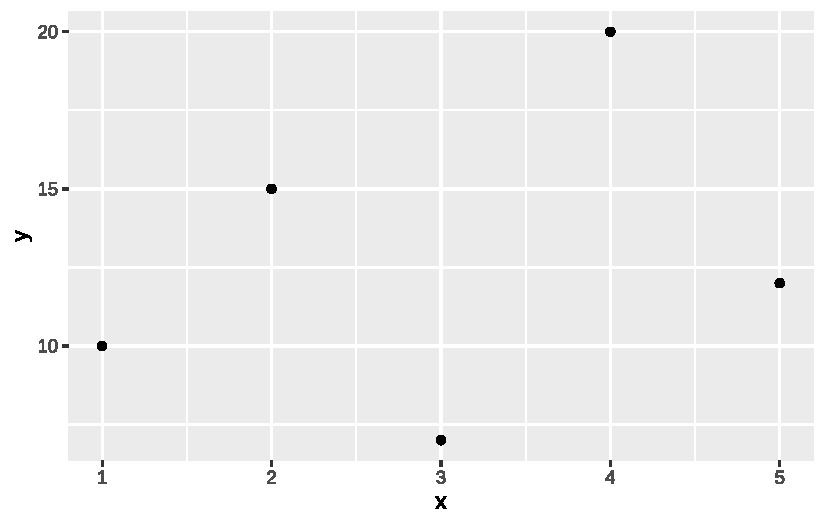
\includegraphics{chapter/base_package_files/figure-pdf/unnamed-chunk-4-1.pdf}

}

\end{figure}

在这个示例中,我们首先加载了\texttt{ggplot2}包,然后创建了一个包含x和y变量的数据框,最后使用\texttt{ggplot2}的函数创建了一个散点图。

\hypertarget{ux5378ux8f7dux5305}{%
\subsection{卸载包}\label{ux5378ux8f7dux5305}}

要卸载一个已安装的包,你可以使用\texttt{remove.packages()}函数。以下是卸载包的步骤:

\begin{enumerate}
\def\labelenumi{\arabic{enumi}.}
\tightlist
\item
  首先,使用\texttt{installed.packages()}函数查看已安装包的列表,找到要卸载的包的名称。
\end{enumerate}

\begin{Shaded}
\begin{Highlighting}[]
\CommentTok{\# 查看已安装的包列表}
\NormalTok{installed\_packages }\OtherTok{\textless{}{-}} \FunctionTok{installed.packages}\NormalTok{()}
\NormalTok{installed\_packages[, }\StringTok{"Package"}\NormalTok{]}
\end{Highlighting}
\end{Shaded}

\begin{verbatim}
                  abind                  ADAPTS                 ambient 
                "abind"                "ADAPTS"               "ambient" 
               ambiorix                annotate           AnnotationDbi 
             "ambiorix"              "annotate"         "AnnotationDbi" 
                anytime                     ape            arrayhelpers 
              "anytime"                   "ape"          "arrayhelpers" 
                  arrow                 arsenal                     aRt 
                "arrow"               "arsenal"                   "aRt" 
            AsioHeaders                 askpass          assertive.base 
          "AsioHeaders"               "askpass"        "assertive.base" 
   assertive.properties         assertive.types                 assertr 
 "assertive.properties"       "assertive.types"               "assertr" 
             assertthat              attachment                 attempt 
           "assertthat"            "attachment"               "attempt" 
                  aweek               backports         bannerCommenter 
                "aweek"             "backports"       "bannerCommenter" 
                   base               base64enc               bayesplot 
                 "base"             "base64enc"             "bayesplot" 
             bayestestR               bdsmatrix                beachmat 
           "bayestestR"             "bdsmatrix"              "beachmat" 
                     BH               BiasedUrn             billboarder 
                   "BH"             "BiasedUrn"           "billboarder" 
                 binman                 Biobase            BiocGenerics 
               "binman"               "Biobase"          "BiocGenerics" 
            BiocManager           BiocNeighbors            BiocParallel 
          "BiocManager"         "BiocNeighbors"          "BiocParallel" 
           BiocSingular             BiocVersion              Biostrings 
         "BiocSingular"           "BiocVersion"            "Biostrings" 
                    bit                   bit64                  bitops 
                  "bit"                 "bit64"                "bitops" 
                   blob                     bmp                 bnlearn 
                 "blob"                   "bmp"               "bnlearn" 
               bnstruct                    boot                     box 
             "bnstruct"                  "boot"                   "box" 
                   brew                    brio                   broom 
                 "brew"                  "brio"                 "broom" 
                bs4Dash                 bsicons                   bslib 
              "bs4Dash"               "bsicons"                 "bslib" 
                 cachem                   Cairo                   callr 
               "cachem"                 "Cairo"                 "callr" 
                    car               carbonate                 carData 
                  "car"             "carbonate"               "carData" 
                  caret                 caTools              cellranger 
                "caret"               "caTools"            "cellranger" 
              checkmate                   chron                   class 
            "checkmate"                 "chron"                 "class" 
               classInt                     cli                   clipr 
             "classInt"                   "cli"                 "clipr" 
                  clock                    clue                 cluster 
                "clock"                  "clue"               "cluster" 
        coarseDataTools                    coda               codetools 
      "coarseDataTools"                  "coda"             "codetools" 
               colormap              colorspace            colourpicker 
             "colormap"            "colorspace"          "colourpicker" 
                 ComICS              commonmark           compareGroups 
               "ComICS"            "commonmark"         "compareGroups" 
               compiler            CompQuadForm                  config 
             "compiler"          "CompQuadForm"                "config" 
             conflicted                 corpcor                corrplot 
           "conflicted"               "corpcor"              "corrplot" 
            countrycode                 cowplot                   cpp11 
          "countrycode"               "cowplot"                 "cpp11" 
                 crayon             credentials               crosstalk 
               "crayon"           "credentials"             "crosstalk" 
                crsmeta                    crul                    curl 
              "crsmeta"                  "crul"                  "curl" 
              cyclocomp                 dagitty              data.table 
            "cyclocomp"               "dagitty"            "data.table" 
         data.validator               DataEditR                datamods 
       "data.validator"             "DataEditR"              "datamods" 
              datapasta                datasets              datawizard 
            "datapasta"              "datasets"            "datawizard" 
                    DBI                  dbplyr                    deal 
                  "DBI"                "dbplyr"                  "deal" 
           DelayedArray      DelayedMatrixStats                  deldir 
         "DelayedArray"    "DelayedMatrixStats"                "deldir" 
             dendextend                DEoptimR                   Deriv 
           "dendextend"              "DEoptimR"                 "Deriv" 
                   desc               DescrTab2               DescTools 
                 "desc"             "DescrTab2"             "DescTools" 
                details                devtools              DiagrammeR 
              "details"              "devtools"            "DiagrammeR" 
          DiagrammeRsvg                   dials              DiceDesign 
        "DiagrammeRsvg"                 "dials"            "DiceDesign" 
                diffobj                  digest          distributional 
              "diffobj"                "digest"        "distributional" 
      DistributionUtils             dockerfiler              doParallel 
    "DistributionUtils"           "dockerfiler"            "doParallel" 
                  doRNG               dotCall64                 downlit 
                "doRNG"             "dotCall64"               "downlit" 
             downloader                   dplyr                   dqrng 
           "downloader"                 "dplyr"                 "dqrng" 
                     DT                  DTedit                  dtplyr 
                   "DT"                "DTedit"                "dtplyr" 
               dygraphs          dynamicTreeCut                   e1071 
             "dygraphs"        "dynamicTreeCut"                 "e1071" 
               eburones               echarts4r          echarts4r.maps 
             "eburones"             "echarts4r"        "echarts4r.maps" 
                  edgeR                editData              effectsize 
                "edgeR"              "editData"            "effectsize" 
          electricShine                 elevatr                 ellipse 
        "electricShine"               "elevatr"               "ellipse" 
               ellipsis                 emmeans                 enrichR 
             "ellipsis"               "emmeans"               "enrichR" 
               EpiEstim                    epiR                esquisse 
             "EpiEstim"                  "epiR"              "esquisse" 
           estimability                evaluate                   Exact 
         "estimability"              "evaluate"                 "Exact" 
               exact2x2                 exactci          exactRankTests 
             "exact2x2"               "exactci"        "exactRankTests" 
                   expm                 ExtDist               extrafont 
                 "expm"               "ExtDist"             "extrafont" 
            extrafontdb              factoextra              FactoMineR 
          "extrafontdb"            "factoextra"            "FactoMineR" 
                  fansi                  farver             fastcluster 
                "fansi"                "farver"           "fastcluster" 
                fastICA                 fastmap                 fdrtool 
              "fastICA"               "fastmap"               "fdrtool" 
                feather                    fftw                  fields 
              "feather"                  "fftw"                "fields" 
                  figma            fitdistrplus              flashClust 
                "figma"          "fitdistrplus"            "flashClust" 
          flexdashboard               flextable                     FNN 
        "flexdashboard"             "flextable"                   "FNN" 
            fontawesome                 forcats                 foreach 
          "fontawesome"               "forcats"               "foreach" 
               forecast                 foreign              forestplot 
             "forecast"               "foreign"            "forestplot" 
                  forge                 formatR                 Formula 
                "forge"               "formatR"               "Formula" 
          formula.tools                fracdiff                   fresh 
        "formula.tools"              "fracdiff"                 "fresh" 
                     fs                     fst                 fstcore 
                   "fs"                   "fst"               "fstcore" 
                  furrr           futile.logger          futile.options 
                "furrr"         "futile.logger"        "futile.options" 
                 future            future.apply               fuzzyjoin 
               "future"          "future.apply"             "fuzzyjoin" 
                    g2r               gapminder                  gargle 
                  "g2r"             "gapminder"                "gargle" 
                  gdata                 gdtools              genefilter 
                "gdata"               "gdtools"            "genefilter" 
                GeneNet   GeneralizedHyperbolic                generics 
              "GeneNet" "GeneralizedHyperbolic"              "generics" 
           GenomeInfoDb        GenomeInfoDbData           GenomicRanges 
         "GenomeInfoDb"      "GenomeInfoDbData"         "GenomicRanges" 
                geojson               geojsonio               geojsonsf 
              "geojson"             "geojsonio"             "geojsonsf" 
             geometries               geosphere                    gert 
           "geometries"             "geosphere"                  "gert" 
                 GGally                   ggdag                  ggdist 
               "GGally"                 "ggdag"                "ggdist" 
                 ggedit               ggeffects                 ggExtra 
               "ggedit"             "ggeffects"               "ggExtra" 
              ggfittext                 ggforce                     ggm 
            "ggfittext"               "ggforce"                   "ggm" 
              ggpattern                 ggplot2                  ggpubr 
            "ggpattern"               "ggplot2"                "ggpubr" 
                 ggraph                 ggrepel                ggridges 
               "ggraph"               "ggrepel"              "ggridges" 
                  ggsci                ggsignif               ggspatial 
                "ggsci"              "ggsignif"             "ggspatial" 
               ggstream                  ggtext           ggThemeAssist 
             "ggstream"                "ggtext"         "ggThemeAssist" 
               ggthemes                  ggvenn               ggvoronoi 
             "ggthemes"                "ggvenn"             "ggvoronoi" 
                     gh                gitcreds                  glasso 
                   "gh"              "gitcreds"                "glasso" 
                    gld                  glmnet                 globals 
                  "gld"                "glmnet"               "globals" 
                   glue                      gm                 gmodels 
                 "glue"                    "gm"               "gmodels" 
                  GO.db                 goftest                   golem 
                "GO.db"               "goftest"                 "golem" 
            googledrive           googlesheets4                   gower 
          "googledrive"         "googlesheets4"                 "gower" 
                  GPfit                  gplots              gptchatteR 
                "GPfit"                "gplots"            "gptchatteR" 
                  graph                graphics            graphlayouts 
                "graph"              "graphics"          "graphlayouts" 
              grDevices                    grid               gridExtra 
            "grDevices"                  "grid"             "gridExtra" 
             gridlayout             gridpattern                gridtext 
           "gridlayout"           "gridpattern"              "gridtext" 
                 gsubfn                  gtable                  gtools 
               "gsubfn"                "gtable"                "gtools" 
                hardhat           HardyWeinberg                   haven 
              "hardhat"         "HardyWeinberg"                 "haven" 
             HDInterval                    here                  hexbin 
           "HDInterval"                  "here"                "hexbin" 
                hexView             highcharter                   highr 
              "hexView"           "highcharter"                 "highr" 
                  Hmisc                     hms              hrbrthemes 
                "Hmisc"                   "hms"            "hrbrthemes" 
              htmlTable               htmltools             htmlwidgets 
            "htmlTable"             "htmltools"           "htmlwidgets" 
               httpcode                  httpuv                    httr 
             "httpcode"                "httpuv"                  "httr" 
                  httr2                humanize                     ica 
                "httr2"              "humanize"                   "ica" 
                    ids                  igraph                  imager 
                  "ids"                "igraph"                "imager" 
                 impute               incidence                   infer 
               "impute"             "incidence"                 "infer" 
             influenceR                     ini                 insight 
           "influenceR"                   "ini"               "insight" 
                 interp                   ipred                 IRanges 
               "interp"                 "ipred"               "IRanges" 
                  irlba                    ISLR                 isoband 
                "irlba"                  "ISLR"               "isoband" 
              iterators               itertools                 janitor 
            "iterators"             "itertools"               "janitor" 
                   jpeg                     jqr               jquerylib 
                 "jpeg"                   "jqr"             "jquerylib" 
                jsonify                jsonlite              kableExtra 
              "jsonify"              "jsonlite"            "kableExtra" 
               KEGGREST                 kernlab              KernSmooth 
             "KEGGREST"               "kernlab"            "KernSmooth" 
                  km.ci                  KMsurv                   knitr 
                "km.ci"                "KMsurv"                 "knitr" 
                     ks                labeling                labelled 
                   "ks"              "labeling"              "labelled" 
               lambda.r                    lars                   later 
             "lambda.r"                  "lars"                 "later" 
              latex2exp                 lattice            latticeExtra 
            "latex2exp"               "lattice"          "latticeExtra" 
                   lava                  lavaan                lazyeval 
                 "lava"                "lavaan"              "lazyeval" 
                    LEA                 leaflet          leaflet.extras 
                  "LEA"               "leaflet"        "leaflet.extras" 
      leaflet.providers                   leaps                  learnr 
    "leaflet.providers"                 "leaps"                "learnr" 
                 leiden                   lemon                     lhs 
               "leiden"                 "lemon"                   "lhs" 
              lifecycle                   limma                   lintr 
            "lifecycle"                 "limma"                 "lintr" 
                listenv              listviewer                    lme4 
              "listenv"            "listviewer"                  "lme4" 
                   lmom                  lmtest                  locfit 
                 "lmom"                "lmtest"                "locfit" 
                    log                  logger            longitudinal 
                  "log"                "logger"          "longitudinal" 
                    loo                   lorem               lubridate 
                  "loo"                 "lorem"             "lubridate" 
                 magick                magrittr                mapplots 
               "magick"              "magrittr"              "mapplots" 
                   maps                maptools                markdown 
                 "maps"              "maptools"              "markdown" 
                   MASS                mathjaxr                  Matrix 
                 "MASS"              "mathjaxr"                "Matrix" 
         MatrixGenerics            MatrixModels             matrixStats 
       "MatrixGenerics"          "MatrixModels"           "matrixStats" 
                maxstat                  mclust                    mcmc 
              "maxstat"                "mclust"                  "mcmc" 
               MCMCpack                     mcp                mdatools 
             "MCMCpack"                   "mcp"              "mdatools" 
                memoise                    meta                 metadat 
              "memoise"                  "meta"               "metadat" 
                metafor               MetBrewer                 methods 
              "metafor"             "MetBrewer"               "methods" 
                   metR                 Metrics                    mgcv 
                 "metR"               "Metrics"                  "mgcv" 
                   mice                    mime                  miniUI 
                 "mice"                  "mime"                "miniUI" 
                  minqa                  misc3d              missForest 
                "minqa"                "misc3d"            "missForest" 
                mitools                 mlbench                  mnormt 
              "mitools"               "mlbench"                "mnormt" 
              modeldata            ModelMetrics                  modelr 
            "modeldata"          "ModelMetrics"                "modelr" 
              mongolite                multcomp               multicool 
            "mongolite"              "multcomp"             "multicool" 
                munsell                 music21                 mvtnorm 
              "munsell"               "music21"               "mvtnorm" 
             NestedMenu               neuralnet                    nlme 
           "NestedMenu"             "neuralnet"                  "nlme" 
                 nloptr                    nnet                    nnls 
               "nloptr"                  "nnet"                  "nnls" 
                nortest                numDeriv                    odbc 
              "nortest"              "numDeriv"                  "odbc" 
                officer                  openai                 openssl 
              "officer"                "openai"               "openssl" 
               openxlsx          operator.tools                  optimx 
             "openxlsx"        "operator.tools"                "optimx" 
                osmdata                  packer                 packrat 
              "osmdata"                "packer"               "packrat" 
                 pacman                     pak                  pander 
               "pacman"                   "pak"                "pander" 
               parallel              parallelly              parameters 
             "parallel"            "parallelly"            "parameters" 
               parsermd                 parsnip               particles 
             "parsermd"               "parsnip"             "particles" 
                pastecs               patchwork                 pbapply 
              "pastecs"             "patchwork"               "pbapply" 
               pbivnorm                pbkrtest                   pcalg 
             "pbivnorm"              "pbkrtest"                 "pcalg" 
                 pcolor                     pcv             performance 
               "pcolor"                   "pcv"           "performance" 
               pheatmap           phosphoricons                  pillar 
             "pheatmap"         "phosphoricons"                "pillar" 
                  pingr                  pinyin                pkgbuild 
                "pingr"                "pinyin"              "pkgbuild" 
              pkgconfig                 pkgdown                 pkgload 
            "pkgconfig"               "pkgdown"               "pkgload" 
                  plogr                  plot3D                  plotly 
                "plogr"                "plot3D"                "plotly" 
                plotrix                     pls                    plyr 
              "plotrix"                   "pls"                  "plyr" 
                    png               polspline                polyclip 
                  "png"             "polspline"              "polyclip" 
                polynom               posterior                  pracma 
              "polynom"             "posterior"                "pracma" 
                 praise          preprocessCore              prettymapr 
               "praise"        "preprocessCore"            "prettymapr" 
            prettyunits                    pROC                processx 
          "prettyunits"                  "pROC"              "processx" 
                prodlim                progress               progressr 
              "prodlim"              "progress"             "progressr" 
                   PROJ                   proj4                promises 
                 "PROJ"                 "proj4"              "promises" 
                  proto               protolite                   proxy 
                "proto"             "protolite"                 "proxy" 
                     ps                   psych                   purrr 
                   "ps"                 "psych"                 "purrr" 
                pushbar                    pzfx                  qgraph 
              "pushbar"                  "pzfx"                "qgraph" 
               quadprog                quantmod                quantreg 
             "quadprog"              "quantmod"              "quantreg" 
                 quarks                  quarto                  qvalue 
               "quarks"                "quarto"                "qvalue" 
                R.cache             R.methodsS3                    R.oo 
              "R.cache"           "R.methodsS3"                  "R.oo" 
                R.utils                    r2d3                      R6 
              "R.utils"                  "r2d3"                    "R6" 
                   ragg            randomForest                  ranger 
                 "ragg"          "randomForest"                "ranger" 
                   RANN              rapidjsonr                rappdirs 
                 "RANN"            "rapidjsonr"              "rappdirs" 
                 raster                rayimage               rayshader 
               "raster"              "rayimage"             "rayshader" 
                   RBGL             rcartocolor              rclipboard 
                 "RBGL"           "rcartocolor"            "rclipboard" 
              rcmdcheck            RColorBrewer                    Rcpp 
            "rcmdcheck"          "RColorBrewer"                  "Rcpp" 
              RcppAnnoy           RcppArmadillo               RcppEigen 
            "RcppAnnoy"         "RcppArmadillo"             "RcppEigen" 
               RcppHNSW            RcppProgress                RcppTOML 
             "RcppHNSW"          "RcppProgress"              "RcppTOML" 
                  RCurl               reactable           reactablefmtr 
                "RCurl"             "reactable"         "reactablefmtr" 
               reactlog                  reactR              readbitmap 
             "reactlog"                "reactR"            "readbitmap" 
                readODS                   readr                  readxl 
              "readODS"                 "readr"                "readxl" 
                recipes              regexplain                 rematch 
              "recipes"            "regexplain"               "rematch" 
               rematch2                 remotes                    renv 
             "rematch2"               "remotes"                  "renv" 
                   repr                  reprex                  reproj 
                 "repr"                "reprex"                "reproj" 
                reshape                reshape2              reticulate 
              "reshape"              "reshape2"            "reticulate" 
                    rex                   rgdal                   rgeos 
                  "rex"                 "rgdal"                 "rgeos" 
                    rgl               Rgraphviz           rhandsontable 
                  "rgl"             "Rgraphviz"         "rhandsontable" 
                  rhino                rintrojs                     rio 
                "rhino"              "rintrojs"                   "rio" 
                  rjags                   rJava                   rjson 
                "rjags"                 "rJava"                 "rjson" 
                RJSONIO                   rlang                   rlist 
              "RJSONIO"                 "rlang"                 "rlist" 
              rmarkdown                  rmatio                     rms 
            "rmarkdown"                "rmatio"                   "rms" 
               rngtools              robustbase                    ROCR 
             "rngtools"            "robustbase"                  "ROCR" 
                  RODBC               rootSolve                    rosm 
                "RODBC"             "rootSolve"                  "rosm" 
               roxygen2                  rpanel                   rpart 
             "roxygen2"                "rpanel"                 "rpart" 
             rpart.plot                    rpdf               RPostgres 
           "rpart.plot"                  "rpdf"             "RPostgres" 
              rprojroot                 rsample               rsconnect 
            "rprojroot"               "rsample"             "rsconnect" 
              RSelenium                  Rsolnp                 RSQLite 
            "RSelenium"                "Rsolnp"               "RSQLite" 
                rstatix              rstudioapi                    rsvd 
              "rstatix"            "rstudioapi"                  "rsvd" 
                   rsvg                   Rtsne                Rttf2pt1 
                 "rsvg"                 "Rtsne"              "Rttf2pt1" 
                 rtweet                 rugarch               rversions 
               "rtweet"               "rugarch"             "rversions" 
                  rvest                      s2               S4Vectors 
                "rvest"                    "s2"             "S4Vectors" 
               sandwich                    sass            ScaledMatrix 
             "sandwich"                  "sass"          "ScaledMatrix" 
                 scales             scattermore           scatterplot3d 
               "scales"           "scattermore"         "scatterplot3d" 
            sctransform                 seewave                 selectr 
          "sctransform"               "seewave"               "selectr" 
                 semver             sessioninfo                settings 
               "semver"           "sessioninfo"              "settings" 
                 Seurat            SeuratObject                      sf 
               "Seurat"          "SeuratObject"                    "sf" 
              sfheaders                 sfsmisc                  shades 
            "sfheaders"               "sfsmisc"                "shades" 
             shadowtext                   shape                   shiny 
           "shadowtext"                 "shape"                 "shiny" 
           shiny.router          shiny.semantic                shinyAce 
         "shiny.router"        "shiny.semantic"              "shinyAce" 
             shinyalert               ShinyAuth                 shinyBS 
           "shinyalert"             "ShinyAuth"               "shinyBS" 
              shinybusy     shinyCopy2clipboard       shinycustomloader 
            "shinybusy"   "shinyCopy2clipboard"     "shinycustomloader" 
         shinydashboard      shinydashboardPlus                shinyDND 
       "shinydashboard"    "shinydashboardPlus"              "shinyDND" 
              shinyjqui                 shinyjs             shinypanels 
            "shinyjqui"               "shinyjs"           "shinypanels" 
               shinysky           shinysnippets             shinythemes 
             "shinysky"         "shinysnippets"           "shinythemes" 
          shinyuieditor            shinyWidgets                showtext 
        "shinyuieditor"          "shinyWidgets"              "showtext" 
             showtextdb                  signal                 SingleR 
           "showtextdb"                "signal"               "SingleR" 
                  sitmo              sjlabelled                  sjmisc 
                "sitmo"            "sjlabelled"                "sjmisc" 
                 sjPlot                 sjstats          SkewHyperbolic 
               "sjPlot"               "sjstats"        "SkewHyperbolic" 
                  skimr                  slider              slippymath 
                "skimr"                "slider"            "slippymath" 
                 smoots               snakecase                    snow 
               "smoots"             "snakecase"                  "snow" 
               sortable             sourcetools                      sp 
             "sortable"           "sourcetools"                    "sp" 
                   spam                sparklyr                 SparseM 
                 "spam"              "sparklyr"               "SparseM" 
      sparseMatrixStats                 spatial           spatstat.data 
    "sparseMatrixStats"               "spatial"         "spatstat.data" 
       spatstat.explore           spatstat.geom         spatstat.random 
     "spatstat.explore"         "spatstat.geom"       "spatstat.random" 
        spatstat.sparse          spatstat.utils                     spd 
      "spatstat.sparse"        "spatstat.utils"                   "spd" 
                splines         splitstackshape                   sqldf 
              "splines"       "splitstackshape"                 "sqldf" 
                SQUAREM                   ssanv               stargazer 
              "SQUAREM"                 "ssanv"             "stargazer" 
                  stats                  stats4              stringdist 
                "stats"                "stats4"            "stringdist" 
                stringi                 stringr             strucchange 
              "stringi"               "stringr"           "strucchange" 
                 styler    SummarizedExperiment                  survey 
               "styler"  "SummarizedExperiment"                "survey" 
               survival               survminer                survMisc 
             "survival"             "survminer"              "survMisc" 
                    sva                 svglite                  svUnit 
                  "sva"               "svglite"                "svUnit" 
                    sys                sysfonts             systemfonts 
                  "sys"              "sysfonts"           "systemfonts" 
                 table1                tableone                   tcltk 
               "table1"              "tableone"                 "tcltk" 
                 tensor                 tensorA                   terra 
               "tensor"               "tensorA"                 "terra" 
           terrainmeshr                testthat             textshaping 
         "terrainmeshr"              "testthat"           "textshaping" 
                TH.data                thematic                  tibble 
              "TH.data"              "thematic"                "tibble" 
                 tictoc               tidybayes               tidygraph 
               "tictoc"             "tidybayes"             "tidygraph" 
               tidyjson              tidymodels                   tidyr 
             "tidyjson"            "tidymodels"                 "tidyr" 
             tidyselect               tidyverse                    tiff 
           "tidyselect"             "tidyverse"                  "tiff" 
             timechange                timeDate                 tinytex 
           "timechange"              "timeDate"               "tinytex" 
                  tippy                   tools            translations 
                "tippy"                 "tools"          "translations" 
             treemapify               triebeard               truncnorm 
           "treemapify"             "triebeard"             "truncnorm" 
                tseries                     TTR                    tune 
              "tseries"                   "TTR"                  "tune" 
                  tuneR                  tweenr                    tzdb 
                "tuneR"                "tweenr"                  "tzdb" 
                  units                    urca                urltools 
                "units"                  "urca"              "urltools" 
                usethis                    utf8                   utils 
              "usethis"                  "utf8"                 "utils" 
                   uuid                    uwot                      V8 
                 "uuid"                  "uwot"                    "V8" 
               validate                    vars                     vcd 
             "validate"                  "vars"                   "vcd" 
                  vctrs                 viridis             viridisLite 
                "vctrs"               "viridis"           "viridisLite" 
             visNetwork                 vistime                   vroom 
           "visNetwork"               "vistime"                 "vroom" 
                  vtree                  waiter                   waldo 
                "vtree"                "waiter"                 "waldo" 
                   warp                   wdman                 webshot 
                 "warp"                 "wdman"               "webshot" 
              websocket                   WGCNA                 whisker 
            "websocket"                 "WGCNA"               "whisker" 
                  withr                      wk               workflows 
                "withr"                    "wk"             "workflows" 
           workflowsets                 writexl                    xfun 
         "workflowsets"               "writexl"                  "xfun" 
                   xlsx                xlsxjars                     XML 
                 "xlsx"              "xlsxjars"                   "XML" 
                   xml2            xmlparsedata                   xopen 
                 "xml2"          "xmlparsedata"                 "xopen" 
                 xtable                     xts                 XVector 
               "xtable"                   "xts"               "XVector" 
                   yaml               yardstick                     yfR 
                 "yaml"             "yardstick"                   "yfR" 
                    zip                zlibbioc                     zoo 
                  "zip"              "zlibbioc"                   "zoo" 
\end{verbatim}

\begin{enumerate}
\def\labelenumi{\arabic{enumi}.}
\setcounter{enumi}{1}
\tightlist
\item
  找到要卸载的包名称后,使用\texttt{remove.packages()}函数进行卸载。假设要卸载名为''mypackage''的包:
\end{enumerate}

\begin{Shaded}
\begin{Highlighting}[]
\CommentTok{\# 卸载包}
\FunctionTok{remove.packages}\NormalTok{(}\StringTok{"mypackage"}\NormalTok{)}
\end{Highlighting}
\end{Shaded}

\hypertarget{ux66f4ux65b0ux5305}{%
\subsection{更新包}\label{ux66f4ux65b0ux5305}}

要更新已安装的包,你可以使用\texttt{update.packages()}函数。以下是更新包的步骤:

\begin{enumerate}
\def\labelenumi{\arabic{enumi}.}
\tightlist
\item
  首先,使用\texttt{update.packages()}函数来检查可用的包更新。这将列出需要更新的包以及它们的版本信息。
\end{enumerate}

\begin{Shaded}
\begin{Highlighting}[]
\CommentTok{\# 检查可用的包更新}
\FunctionTok{update.packages}\NormalTok{(}\AttributeTok{ask =} \ConstantTok{FALSE}\NormalTok{)}
\end{Highlighting}
\end{Shaded}

\begin{enumerate}
\def\labelenumi{\arabic{enumi}.}
\setcounter{enumi}{1}
\tightlist
\item
  如果你希望更新所有可用的包,可以在\texttt{update.packages()}函数中设置\texttt{ask}参数为\texttt{FALSE},然后运行函数。
\end{enumerate}

\begin{Shaded}
\begin{Highlighting}[]
\CommentTok{\# 更新所有可用的包(不询问)}
\FunctionTok{update.packages}\NormalTok{(}\AttributeTok{ask =} \ConstantTok{FALSE}\NormalTok{)}
\end{Highlighting}
\end{Shaded}

\begin{enumerate}
\def\labelenumi{\arabic{enumi}.}
\setcounter{enumi}{2}
\tightlist
\item
  如果你只想更新特定的包,可以提供包名称的向量作为参数。例如,要更新''ggplot2''和''dplyr''包:
\end{enumerate}

\begin{Shaded}
\begin{Highlighting}[]
\CommentTok{\# 更新特定的包}
\FunctionTok{update.packages}\NormalTok{(}\AttributeTok{ask =} \ConstantTok{FALSE}\NormalTok{, }\AttributeTok{lib.loc =} \FunctionTok{.libPaths}\NormalTok{(), }\AttributeTok{oldPkgs =} \FunctionTok{c}\NormalTok{(}\StringTok{"ggplot2"}\NormalTok{, }\StringTok{"dplyr"}\NormalTok{))}
\end{Highlighting}
\end{Shaded}

上述方法允许你卸载和更新R包,确保你的R环境中始终使用最新版本的包。在数据分析和编程中,定期更新包非常重要,因为更新通常包含了错误修复和新功能。

\hypertarget{ux6700ux4f73ux63a8ux8350-rioux5305}{%
\chapter{最佳推荐-rio包}\label{ux6700ux4f73ux63a8ux8350-rioux5305}}

\begin{Shaded}
\begin{Highlighting}[]
\FunctionTok{library}\NormalTok{(rio)}
\end{Highlighting}
\end{Shaded}

\part{数据清理}

\hypertarget{section}{%
\chapter{}\label{section}}

\hypertarget{ux4ecbux7ecd}{%
\chapter{介绍}\label{ux4ecbux7ecd}}

\texttt{dplyr}是一个R语言包,它提供了一组用于进行数据操作和转换的函数。下面是一些\texttt{dplyr}包中常用的函数及其作用:

\begin{itemize}
\tightlist
\item
  \texttt{mutate()}: 创建新的计算变量
\item
  \texttt{filter()}: 根据条件选择行
\item
  \texttt{select()}: 选择列
\item
  \texttt{arrange()}: 按照指定的列排序
\item
  \texttt{distinct()}: 选择唯一的行
\item
  \texttt{summarize()}: 计算每组数据的摘要统计量
\item
  \texttt{group\_by()}: 按照指定的列对数据进行分组
\item
  \texttt{join()}: 将多个表格合并成一个表格
\item
  \texttt{union()}: 将两个表格合并为一个表格(类似于SQL中的UNION)
\item
  \texttt{intersect()}: 取两个表格的交集(类似于SQL中的INTERSECT)
\item
  \texttt{anti\_join()}: 取两个表格的差集(类似于SQL中的EXCEPT)
\end{itemize}

\#\#mutate()

\texttt{mutate()}是\texttt{dplyr}包中的一个函数,用于创建新的计算变量。例如,假设你有一个名为\texttt{data}的数据框,其中包含一列名为\texttt{x}和一列名为\texttt{y},你可以用以下代码创建一个新的列\texttt{z},其值为\texttt{x}和\texttt{y}的和:

\begin{verbatim}
data <- mutate(data, z = x + y)
\end{verbatim}

你可以用类似的方式创建其他任何计算变量。例如,你可以根据条件创建一个分类变量:

\begin{verbatim}
data <- mutate(data, group = ifelse(x > 0, "positive", "negative"))
\end{verbatim}

另外,你也可以在\texttt{mutate()}函数中使用其他函数,例如聚合函数或统计函数,来对原数据进行处理。例如,你可以计算每个\texttt{x}值的均值和标准差:

\begin{verbatim}
data <- mutate(data,
  x_mean = mean(x),
  x_sd = sd(x)
)
\end{verbatim}

你还可以使用\texttt{group\_by()}函数来根据指定的列对数据进行分组,然后在每组中应用\texttt{mutate()}函数,以便为每个组分别计算新的变量。例如:

\begin{verbatim}
data <- group_by(data, group) %>%
  mutate(
    x_mean = mean(x),
    x_sd = sd(x)
  )
\end{verbatim}

\hypertarget{select}{%
\section{select()}\label{select}}

\texttt{select()}是\texttt{dplyr}包中的一个函数,它用于选择数据框中的特定列。例如,假设你有一个名为\texttt{data}的数据框,其中包含多列,你可以用以下代码选择列\texttt{x}和列\texttt{y}:

\begin{verbatim}
data <- select(data, x, y)
\end{verbatim}

在这个例子中,\texttt{select()}函数会返回一个新的数据框,其中只包含原来数据框中的列\texttt{x}和列\texttt{y}。你也可以使用通配符来选择多个列。例如:

\begin{verbatim}
data <- select(data, starts_with("x"))
\end{verbatim}

这里的\texttt{starts\_with()}函数会匹配所有以\texttt{x}开头的列名,例如\texttt{x1}、\texttt{x2}等,然后\texttt{select()}函数会返回一个新的数据框,其中包含原数据框中所有以\texttt{x}开头的列。

除了选择列,你还可以用\texttt{select()}函数来排除列。例如:

\begin{verbatim}
data <- select(data, -z)
\end{verbatim}

这里,我们使用了负号(\texttt{-})来排除列\texttt{z},\texttt{select()}函数会返回一个新的数据框,其中包含原数据框中除列\texttt{z}以外的所有列。

你也可以使用类似的方式来排除多个列,例如:

\begin{verbatim}
data <- select(data, -starts_with("x"))
\end{verbatim}

这里,我们使用了\texttt{starts\_with()}函数来匹配所有以\texttt{x}开头的列名,然后用负号排除这些列。\texttt{select()}函数会返回一个新的数据框,其中包含原数据框中除了以\texttt{x}开头的列以外的所有列。

除了使用函数来选择或排除列,你还可以使用类似于SQL中的语法来指定要选择或排除的列。例如:

\begin{verbatim}
data <- select(data, x, y, -z)
\end{verbatim}

这里,我们指定了要选择列\texttt{x}和列\texttt{y},并使用负号排除列\texttt{z}。\texttt{select()}函数会返回一个新的数据框,其中包含原数据框中的列\texttt{x}、列\texttt{y},除列\texttt{z}以外的所有列。

\hypertarget{ux9009ux62e9ux5668ux51fdux6570ux6709ux54eaux4e9b}{%
\subsection{选择器函数有哪些}\label{ux9009ux62e9ux5668ux51fdux6570ux6709ux54eaux4e9b}}

在 \texttt{tidyverse}
语法中,有多种选择器函数可以用来选择数据框中的特定列。这些选择器函数主要有如下几种:

\begin{itemize}
\tightlist
\item
  \texttt{starts\_with()}:选择名称以某个字符串开头的列。
\item
  \texttt{ends\_with()}:选择名称以某个字符串结尾的列。
\item
  \texttt{contains()}:选择名称中包含某个字符串的列。
\item
  \texttt{matches()}:选择名称与某个正则表达式相匹配的列。
\item
  \texttt{one\_of()}:选择名称在指定列表中出现过的列。
\item
  \texttt{everything()}:选择所有列。
\end{itemize}

例如,如果您想要选择 \texttt{my\_data} 数据框中名称以 \texttt{age}
开头的列,可以使用如下语句:

\begin{verbatim}
Copy codemy_data_selected <- my_data %>% select(starts_with("age"))
\end{verbatim}

这条语句的意思是,在 \texttt{my\_data} 数据框中选择名称以 \texttt{age}
开头的列,并将结果保存到变量 \texttt{my\_data\_selected} 中。

如果您想要选择 \texttt{my\_data} 数据框中名称以 \texttt{age} 结尾的列。

如果您想要选择 \texttt{my\_data} 数据框中名称以 \texttt{age}
结尾的列,可以使用如下语句:

\begin{verbatim}
my_data_selected <- my_data %>% select(ends_with("age"))
\end{verbatim}

如果您想要选择 \texttt{my\_data} 数据框中名称中包含 \texttt{age}
的列,可以使用如下语句:

\begin{verbatim}
my_data_selected <- my_data %>% select(contains("age"))
\end{verbatim}

如果您想要选择 \texttt{my\_data} 数据框中名称与正则表达式 \texttt{"a.e"}
相匹配的列,可以使用如下语句:

\begin{verbatim}
my_data_selected <- my_data %>% select(matches("a.e"))
\end{verbatim}

如果您想要选择 \texttt{my\_data} 数据框中名称在列表
\texttt{c("age",\ "height")} 中出现过的列,可以使用如下语句:

\begin{verbatim}
my_data_selected <- my_data %>% select(one_of(c("age", "height")))
\end{verbatim}

如果您想要选择 \texttt{my\_data} 数据框中的所有列,可以使用如下语句:

\begin{verbatim}
my_data_selected <- my_data %>% select(everything())
\end{verbatim}

\hypertarget{ux5176ux4ed6ux7684ux9009ux62e9ux5668ux51fdux6570}{%
\subsection{其他的选择器函数}\label{ux5176ux4ed6ux7684ux9009ux62e9ux5668ux51fdux6570}}

除了以上提到的选择器函数,\texttt{tidyverse}
语法中还有一些其他选择器函数可以用来选择数据框中的特定列。例如,还有以下几种常用的选择器函数:

\begin{itemize}
\tightlist
\item
  \texttt{num\_range()}:选择名称在指定数字范围内的列。
\item
  \texttt{cols()}:选择指定的列。
\item
  \texttt{which()}:选择满足某个条件的列。
\end{itemize}

例如,如果您想要选择 \texttt{my\_data} 数据框中名称在数字范围 {[}1,5{]}
内的列,可以使用如下语句:

\begin{verbatim}
my_data_selected <- my_data %>% select(num_range(1, 5))
\end{verbatim}

如果您想要选择 \texttt{my\_data} 数据框中指定的列,可以使用如下语句:

\begin{verbatim}
my_data_selected <- my_data %>% select(cols(age, height))
\end{verbatim}

这条语句的意思是,在 \texttt{my\_data} 数据框中选择 \texttt{age} 和
\texttt{height} 两列,并将结果保存到变量 \texttt{my\_data\_selected}
中。

如果您想要选择 \texttt{my\_data}
数据框中满足某个条件的列,可以使用如下语句:

\begin{verbatim}
my_data_selected <- my_data %>% select(which(colnames(my_data) %in% c("age", "height")))
\end{verbatim}

这条语句的意思是,在 \texttt{my\_data} 数据框中选择名称在列表
\texttt{c("age",\ "height")} 中出现过的列,并将结果保存到变量
\texttt{my\_data\_selected} 中。

通过使用上述语句,您可以方便地选择数据框中的特定列。更多关于选择器函数的信息,可以参考
\texttt{tidyverse} 官方文档。

\hypertarget{matchux9009ux62e9ux5668ux51fdux6570ux4e2dux7684ux6b63ux5219ux8868ux8fbeux5f0f}{%
\subsection{match选择器函数中的正则表达式}\label{matchux9009ux62e9ux5668ux51fdux6570ux4e2dux7684ux6b63ux5219ux8868ux8fbeux5f0f}}

在 \texttt{match()}
选择器函数中,您可以使用正则表达式来匹配列名。正则表达式的语法与 R
语言的其他用法相同,详细内容可以参考 R 语言的官方文档。

一般来说,您可以使用以下一些常用语法来构造正则表达式:

\begin{itemize}
\item
  \texttt{.}:表示任意一个字符。例如,正则表达式 \texttt{"a.c"}
  可以匹配列名为 \texttt{"abc"}、\texttt{"aac"} 等。
\item
  \texttt{*}:表示前面的字符可以重复出现任意次。例如,正则表达式
  \texttt{"a*c"} 可以匹配列名为
  \texttt{"c"}、\texttt{"ac"}、\texttt{"aaac"} 等。
\item
  \texttt{+}:表示前面的字符必须至少出现一次。例如,正则表达式
  \texttt{"a+c"} 可以匹配列名为
  \texttt{"ac"}、\texttt{"aac"}、\texttt{"aaac"} 等,但不能匹配列名为
  \texttt{"c"}。
\item
  \texttt{\^{}}:表示以某个字符串开头。例如,正则表达式 \texttt{"\^{}a"}
  可以匹配列名为 \texttt{"abc"}、\texttt{"ac"} 等,但不能匹配列名为
  \texttt{"bc"}。
\item
  \texttt{\$}:表示以某个字符串结尾。例如,正则表达式 \texttt{"c\$"}
  可以匹配列名为 \texttt{"abc"}、\texttt{"ac"} 等,但不能匹配列名为
  \texttt{"bc"}。
\end{itemize}

除了以上语法,正则表达式还有很多其他用法。

\hypertarget{ux6b63ux5219ux8868ux8fbeux5f0fux7684ux9ad8ux7ea7ux8bedux6cd5ux6709ux54eaux4e9b}{%
\subsection{正则表达式的高级语法有哪些}\label{ux6b63ux5219ux8868ux8fbeux5f0fux7684ux9ad8ux7ea7ux8bedux6cd5ux6709ux54eaux4e9b}}

除了以上提到的正则表达式的基本语法,还有一些高级语法可以用来构造更复杂的正则表达式。例如,您可以使用以下一些常用语法来构造正则表达式:

\begin{itemize}
\tightlist
\item
  \texttt{\textbar{}}:表示或的关系。例如,正则表达式
  \texttt{"a\textbar{}b"} 可以匹配列名为 \texttt{"a"}、\texttt{"b"} 等。
\item
  \texttt{{[}{]}}:表示括号中的任意一个字符。例如,正则表达式
  \texttt{"{[}ab{]}"} 可以匹配列名为 \texttt{"a"}、\texttt{"b"} 等。
\item
  \texttt{{[}a-z{]}}:表示小写字母 a 到 z
  中的任意一个字符。例如,正则表达式 \texttt{"{[}a-z{]}"} 可以匹配列名为
  \texttt{"a"}、\texttt{"b"}、\texttt{"c"} 等。
\item
  \texttt{{[}A-Z{]}}:表示大写字母 A 到 Z
  中的任意一个字符。例如,正则表达式 \texttt{"{[}A-Z{]}"} 可以匹配列名为
  \texttt{"A"}、\texttt{"B"}、\texttt{"C"} 等。
\item
  \texttt{\textbackslash{}\textbackslash{}d}:表示任意一个数字。例如,正则表达式
  \texttt{"\textbackslash{}\textbackslash{}d"} 可以匹配列名为
  \texttt{"1"}、\texttt{"2"}、\texttt{"3"} 等。
\end{itemize}

除了以上语法,正则表达式还有很多其他高级语法。您可以参考 R
语言的官方文档或相关资料来了解更多信息。

\hypertarget{filter}{%
\section{filter()}\label{filter}}

\texttt{filter()}是\texttt{dplyr}包中的一个函数,它用于根据指定的条件选择数据框中的行。例如,假设你有一个名为\texttt{data}的数据框,其中包含多行多列,你可以用以下代码选择值大于0的行:

\begin{verbatim}
data <- filter(data, x > 0)
\end{verbatim}

在这个例子中,\texttt{filter()}函数会返回一个新的数据框,其中只包含原数据框中值大于0的行。你也可以使用多个条件来进行筛选。例如:

\begin{verbatim}
data <- filter(data, x > 0, y < 5)
\end{verbatim}

这里,\texttt{filter()}函数会返回一个新的数据框,其中只包含原数据框中值大于0且值小于5的行。

除了简单的条件判断,你还可以在\texttt{filter()}函数中使用复杂的逻辑表达式来进行筛选。例如:

\begin{verbatim}
data <- filter(data, x > 0 & y < 5 | z == 0)
\end{verbatim}

这里,我们使用了与(\texttt{\&})、或(\texttt{\textbar{}})以及等于(\texttt{==})符号来构造复杂的逻辑表达式,\texttt{filter()}函数会返回一个新的数据框,其中只包含原数据框中符合

\hypertarget{group_by}{%
\section{group\_by()}\label{group_by}}

\texttt{group\_by()} 是 dplyr
包中的一个函数,它能够将数据按照指定的条件进行分组。通常,我们使用
\texttt{group\_by()}
函数将数据按照某个变量的值进行分组,然后再对每个分组进行进一步的操作。

例如,假设我们有一个数据框 \texttt{my\_data},它包含两个变量,分别为
\texttt{name} 和 \texttt{age}。如果我们想要将数据框 \texttt{my\_data}
按照 \texttt{age} 变量的值进行分组,可以使用如下语句:

\begin{verbatim}
my_data_grouped <- group_by(my_data, age)
\end{verbatim}

这条语句的意思是,使用 \texttt{group\_by()} 函数将数据框
\texttt{my\_data} 按照 \texttt{age} 变量的值进行分组,并将结果保存到变量
\texttt{my\_data\_grouped} 中。

接下来,我们可以对每个分组进行进一步的操作。例如,如果我们想要计算每个分组中
\texttt{name} 变量的平均值,可以使用 \texttt{summarise()} 函数来实现:

\begin{verbatim}
my_data_summary <- summarise(
  my_data_grouped, 
  mean_name = mean(name))
\end{verbatim}

这条语句的意思是,对分组后的数据框 \texttt{my\_data\_grouped}
中的每个分组,计算 \texttt{name} 变量的平均值。

\hypertarget{ux591aux7ea7ux5206ux7ec4}{%
\subsection{多级分组}\label{ux591aux7ea7ux5206ux7ec4}}

当然,您也可以使用 \texttt{group\_by()}
函数进行多级分组。例如,如果您想要将数据框 \texttt{my\_data} 按照
\texttt{age} 和 \texttt{height}
两个变量的值进行多级分组,可以使用如下语句:

\begin{verbatim}
Copy codemy_data_grouped <- group_by(my_data, age, height, .drop = F)
\end{verbatim}

这条语句的意思是,按照 \texttt{age} 和 \texttt{height}
两个变量的值进行多级分组,并将结果保存到变量 \texttt{my\_data\_grouped}
中。

在这个例子中,我们还使用了 \texttt{.drop} 参数,它的值设置为
\texttt{F}。这个参数的作用是,是否将分组后的数据框中不重要的列去掉。如果将
\texttt{.drop} 参数设置为 \texttt{T},那么 R
会去掉分组后的数据框中不重要的列。如果将 \texttt{.drop} 参数设置为
\texttt{F},则保留分组后的数据框中的所有列。

在使用 \texttt{group\_by()}
函数时,可以根据实际情况来调整分组条件和参数的值,以实现不同的分组效果。不管是单级分组还是多级分组,

\hypertarget{ux91cdux65b0ux5206ux7ec4}{%
\subsection{重新分组}\label{ux91cdux65b0ux5206ux7ec4}}

如果您想要对已经分组的数据进行重新分组,可以再次使用
\texttt{group\_by()} 函数。例如,假设您已经将数据框 \texttt{my\_data}
按照 \texttt{age} 变量的值进行分组,并将结果保存到变量
\texttt{my\_data\_grouped} 中,如果您想要按照 \texttt{height}
变量的值进行重新分组,可以使用如下语句:

\begin{verbatim}
my_data_grouped <- group_by(my_data_grouped, height)
\end{verbatim}

这条语句的意思是,对已经分组的数据框 \texttt{my\_data\_grouped} 按照
\texttt{height} 变量的值进行重新分组,并将结果保存到变量
\texttt{my\_data\_grouped} 中。

\hypertarget{ux53d6ux6d88ux5206ux7ec4}{%
\subsection{取消分组}\label{ux53d6ux6d88ux5206ux7ec4}}

如果您想要取消分组,可以使用 \texttt{ungroup()}
函数。例如,假设您已经将数据框 \texttt{my\_data} 按照 \texttt{age}
变量的值进行分组,并将结果保存到变量 \texttt{my\_data\_grouped}
中,如果您想要取消分组,可以使用如下语句:

\begin{verbatim}
my_data_ungrouped <- ungroup(my_data_grouped)
\end{verbatim}

这条语句的意思是,对分组后的数据框 \texttt{my\_data\_grouped}
进行取消分组操作,并将结果保存到变量 \texttt{my\_data\_ungrouped} 中。

取消分组后,数据框会恢复到未分组的状态。

\hypertarget{summarise}{%
\section{summarise()}\label{summarise}}

\texttt{summarise()}是\texttt{dplyr}包中的一个函数,它用于对数据框进行汇总。例如,假设你有一个名为\texttt{data}的数据框,其中包含多行多列,你可以用以下代码计算每个组的均值:

\begin{verbatim}
data <- group_by(data, group) %>%
  summarise(mean = mean(x))
\end{verbatim}

在这个例子中,我们首先使用\texttt{group\_by()}函数将数据框按照列\texttt{group}进行分组,然后使用\texttt{summarise()}函数计算每个组的均值。\texttt{summarise()}函数会返回一个新的数据框,其中包含每个组的均值以及对应的组名。

除了计算均值,你还可以使用\texttt{summarise()}函数计算其他统计量,例如求和、求最大值求最小值等。例如:

\begin{verbatim}
data <- group_by(data, group) %>%
  summarise(sum = sum(x),
            max = max(x),
            min = min(x))
\end{verbatim}

在这个例子中,我们首先将数据框按照列\texttt{group}进行分组,然后使用\texttt{summarise()}函数计算每个组的和、最大值和最小值。\texttt{summarise()}函数会返回一个新的数据框,其中包含每个组的和、最大值和最小值以及对应的组名。

\hypertarget{distinct}{%
\section{distinct()}\label{distinct}}

\texttt{distinct()} 函数是 \texttt{tidyverse}
包中的一个函数,用于选择指定数据框中不同的行。例如,如果您想要从
\texttt{my\_data} 数据框中选择出不同的行,可以使用如下语句:

\begin{verbatim}
my_data_distinct <- my_data %>% distinct()
\end{verbatim}

这条语句的意思是,在 \texttt{my\_data}
数据框中选择出不同的行,并将结果保存到变量 \texttt{my\_data\_distinct}
中。

除了上述语句,您还可以使用 \texttt{distinct()}
函数指定选择哪些列来检查行的唯一性。例如,如果您想要仅以 \texttt{age}
列为依据来选择不同的行,可以使用如下语句:

\begin{verbatim}
my_data_distinct <- my_data %>% distinct(age)
\end{verbatim}

这条语句的意思是,在 \texttt{my\_data} 数据框中选择出不同的行,并仅以
\texttt{age} 列为依据来检查行的唯一性。由于这条语句只检查了 \texttt{age}
列,所以如果两行中 \texttt{age}
列的值相同,那么这两行都会被认为是重复的,只会保留一行。最终的结果会被保存到变量
\texttt{my\_data\_distinct} 中。

另外,您还可以使用 \texttt{distinct()} 函数中的 \texttt{.keep\_all}
参数来指定是否保留所有列。例如,如果您想要保留所有列,可以使用如下语句:

\begin{verbatim}
my_data_distinct <- my_data %>% distinct(.keep_all = TRUE)
\end{verbatim}

这条语句的意思是,在 \texttt{my\_data}
数据框中选择出不同的行,并保留所有列。由于这条语句指定了
\texttt{.keep\_all\ =\ TRUE}
参数,所以所有的列都会被保留。最终的结果会被保存到变量
\texttt{my\_data\_distinct} 中。

\hypertarget{arrange}{%
\section{arrange()}\label{arrange}}

\texttt{arrange()} 函数是 \texttt{tidyverse}
包中的一个函数,用于对指定数据框中的行进行排序。例如,如果您想要对
\texttt{my\_data} 数据框中的行按照 \texttt{age}
列的值进行排序,可以使用如下语句:

\begin{verbatim}
my_data_arranged <- my_data %>% arrange(age)
\end{verbatim}

这条语句的意思是,在 \texttt{my\_data} 数据框中按照 \texttt{age}
列的值进行排序,并将结果保存到变量 \texttt{my\_data\_arranged} 中。

除了上述语句,您还可以使用 \texttt{arrange()} 函数中的 \texttt{desc()}
函数来指定是否按照降序进行排序。例如,如果您想要按照降序排序,可以使用如下语句:

\begin{verbatim}
my_data_arranged <- my_data %>% 
  arrange(desc(age))
\end{verbatim}

这条语句的意思是,在 \texttt{my\_data} 数据框中按照 \texttt{age}
列的值按照降序进行排序,并将结果保存到变量 \texttt{my\_data\_arranged}
中。

另外,您还可以使用 \texttt{arrange()} 函数中的 \texttt{dplyr::first()}
函数来选择每组第一行。例如,如果您想要选择每组第一行,可以使用如下语句:

\begin{verbatim}
my_data_arranged <- my_data %>% arrange(group, dplyr::first())
\end{verbatim}

这条语句的意思是,在 \texttt{my\_data} 数据框中按照 \texttt{group}
列的值进行分组,并选择每组第一行。最终的结果会被保存到变量
\texttt{my\_data\_arranged} 中。

除了以上语句,您还可以使用 \texttt{arrange()} 函数中的
\texttt{dplyr::last()}
函数来选择每组最后一行。例如,如果您想要选择每组最后一行,可以使用如下语句:

\begin{verbatim}
my_data_arranged <- my_data %>% 
  arrange(group, dplyr::last())
\end{verbatim}

这条语句的意思是,在 \texttt{my\_data} 数据框中按照 \texttt{group}
列的值进行分组,并选择每组最后一行。最终的结果会被保存到变量
\texttt{my\_data\_arranged} 中。

另外,您还可以使用 \texttt{arrange()} 函数中的 \texttt{dplyr::nth()}
函数来选择每组的指定行。例如,如果您想要选择每组的第二行,可以使用如下语句:

\begin{verbatim}
my_data_arranged <- my_data %>% 
  arrange(group, dplyr::nth(2))
\end{verbatim}

这条语句的意思是,在 \texttt{my\_data} 数据框中按照 \texttt{group}
列的值进行分组,并选择每组的第二行。最终的结果会被保存到变量
\texttt{my\_data\_arranged} 中。

\hypertarget{section-1}{%
\chapter{}\label{section-1}}

\hypertarget{ux4ecbux7ecd-1}{%
\chapter{介绍}\label{ux4ecbux7ecd-1}}

\texttt{stringr}
包包含了许多实用的函数,这些函数可以用来处理字符串。下面是
\texttt{stringr} 包中一些常用的函数及其作用:

\begin{itemize}
\tightlist
\item
  \texttt{str\_length()}
  函数:可以计算字符串的长度(即字符串中字符的数量)。
\item
  \texttt{str\_replace()} 函数:可以替换字符串中的某个部分。
\item
  \texttt{str\_detect()} 函数:可以检测字符串中是否包含某个指定的子串。
\item
  \texttt{str\_count()} 函数:可以计算字符串中包含某个指定的子串的数量。
\item
  \texttt{str\_split()}
  函数:可以根据指定的分隔符将字符串分割成多个子串。
\item
  \texttt{str\_c()} 函数:可以将多个字符串拼接成一个字符串。
\item
  \texttt{str\_to\_lower()} 函数:可以将字符串中的所有字符转换为小写。
\item
  \texttt{str\_to\_upper()} 函数:可以将字符串中的所有字符转换为大写。
\end{itemize}

\hypertarget{str_length}{%
\section{str\_length()}\label{str_length}}

\texttt{str\_length()} 函数是 \texttt{stringr}
包中的一个函数,用于计算字符串的长度(即字符串中字符的数量)。例如,下面的代码使用
\texttt{str\_length()} 函数来计算字符串的长度:

\begin{verbatim}
# 加载 stringr 包
library(stringr)

# 定义一个字符串
my_string <- "Hello, world!"

# 使用 str_length() 函数来计算字符串的长度
my_string_length <- str_length(my_string)

# 输出结果
print(my_string_length)
\end{verbatim}

运行上面的代码后,可以在 R 终端中看到输出的结果:

\begin{verbatim}
[1] 13
\end{verbatim}

这表明,字符串 ``Hello, world!'' 的长度为 13(包含 13 个字符)。

\hypertarget{str_replace}{%
\section{str\_replace()}\label{str_replace}}

\texttt{str\_replace()} 函数是 \texttt{stringr}
包中的一个函数,用于替换字符串中的某个部分。该函数的语法格式如下:

\begin{verbatim}
str_replace(string, pattern, replacement)
\end{verbatim}

其中,\texttt{string} 是要进行替换操作的字符串,\texttt{pattern}
是要替换的子串,\texttt{replacement}
是用来替换的新子串。例如,下面的代码使用 \texttt{str\_replace()}
函数来替换字符串中的某个部分:

\begin{verbatim}
# 加载 stringr 包
library(stringr)

# 定义一个字符串
my_string <- "Hello, world!"

# 使用 str_replace() 函数来替换字符串中的某个部分
my_string_replaced <- str_replace(my_string, "world", "R")

# 输出结果
print(my_string_replaced)
\end{verbatim}

运行上面的代码后,可以在 R 终端中看到输出的结果:

\begin{verbatim}
[1] "Hello, R!"
\end{verbatim}

\hypertarget{str_detect}{%
\section{str\_detect()}\label{str_detect}}

\texttt{str\_detect()} 函数是 \texttt{stringr}
包中的一个函数,用于检测字符串中是否包含某个指定的子串。该函数的语法格式如下:

\begin{verbatim}
str_detect(string, pattern)
\end{verbatim}

其中,\texttt{string} 是要检测的字符串,\texttt{pattern}
是要查找的子串。例如,下面的代码使用 \texttt{str\_detect()}
函数来检测字符串中是否包含某个指定的子串:

\begin{verbatim}
# 加载 stringr 包
library(stringr)

# 定义一个字符串
my_string <- "Hello, world!"

# 使用 str_detect() 函数来检测字符串中是否包含某个指定的子串
is_substring_present <- str_detect(my_string, "world")

# 输出结果
print(is_substring_present)
\end{verbatim}

运行上面的代码后,可以在 R 终端中看到输出的结果:

\begin{verbatim}
[1] TRUE
\end{verbatim}

这表明,字符串 ``Hello, world!'' 中包含了子串 ``world''。

\hypertarget{str_count}{%
\section{str\_count()}\label{str_count}}

\texttt{str\_count()} 函数是 \texttt{stringr}
包中的一个函数,用于统计字符串中某个子串的出现次数。该函数的语法格式如下:

\begin{verbatim}
str_count(string, pattern)
\end{verbatim}

其中,\texttt{string} 是要检测的字符串,\texttt{pattern}
是要查找的子串。例如,下面的代码使用 \texttt{str\_count()}
函数来统计字符串中某个子串的出现次数:

\begin{verbatim}
# 加载 stringr 包
library(stringr)

# 定义一个字符串
my_string <- "Hello, world!"

# 使用 str_count() 函数来统计字符串中某个子串的出现次数
my_string_count <- str_count(my_string, "l")

# 输出结果
print(my_string_count)
\end{verbatim}

运行上面的代码后,可以在 R 终端中看到输出的结果:

\begin{verbatim}
[1] 3
\end{verbatim}

这表明,字符串 ``Hello, world!'' 中子串 ``l'' 出现了 3 次。

\hypertarget{str_split}{%
\section{str\_split()}\label{str_split}}

\texttt{str\_split()} 函数是 \texttt{stringr}
包中的一个函数,用于将字符串按照指定的分隔符进行分割,并返回一个字符串数组。该函数的语法格式如下:

\begin{verbatim}
str_split(string, pattern)
\end{verbatim}

其中,\texttt{string} 是要分割的字符串,\texttt{pattern}
是用来分割字符串的分隔符。例如,下面的代码使用 \texttt{str\_split()}
函数来将字符串按照逗号进行分割:

\begin{verbatim}
# 加载 stringr 包
library(stringr)

# 定义一个字符串
my_string <- "Hello, world!"

# 使用 str_split() 函数将字符串按照逗号进行分割
my_string_split <- str_split(my_string, ",")

# 输出结果
print(my_string_split)
\end{verbatim}

运行上面的代码后,可以在 R 终端中看到输出的结果:

\begin{verbatim}
[[1]]
[1] "Hello" " world!"
\end{verbatim}

这表明,字符串 ``Hello, world!''
被按照逗号进行分割后,得到了包含两个元素的字符串数组,分别为 ``Hello''
和 '' world!{}``。

\hypertarget{str_c}{%
\section{str\_c()}\label{str_c}}

\texttt{str\_c()} 函数是 \texttt{stringr}
包中的一个函数,用于将多个字符串拼接成一个新的字符串。该函数的语法格式如下:

\begin{verbatim}
str_c(..., sep = "")
\end{verbatim}

其中,\texttt{...} 表示可以传入任意多个字符串,\texttt{sep}
参数表示分隔符,即拼接后的字符串中,每两个字符串之间的分隔符。例如,下面的代码使用
\texttt{str\_c()} 函数来将多个字符串拼接成一个新的字符串:

\begin{verbatim}
# 加载 stringr 包
library(stringr)

# 使用 str_c() 函数将多个字符串拼接成一个新的字符串
my_string <- str_c("Hello", "world", "!")

# 输出结果
print(my_string)
\end{verbatim}

运行上面的代码后,可以在 R 终端中看到输出的结果:

\begin{verbatim}
[1] "Helloworld!"
\end{verbatim}

\hypertarget{str_to_lower}{%
\section{str\_to\_lower()}\label{str_to_lower}}

\texttt{str\_to\_lower()} 函数是 \texttt{stringr}
包中的一个函数,用于将字符串中的所有字母转换为小写字母。该函数的语法格式如下:

\begin{verbatim}
str_to_lower(string)
\end{verbatim}

其中,\texttt{string} 是要转换的字符串。例如,下面的代码使用
\texttt{str\_to\_lower()} 函数将字符串中的所有字母转换为小写字母:

\begin{verbatim}
# 加载 stringr 包
library(stringr)

# 定义一个字符串
my_string <- "Hello, world!"

# 使用 str_to_lower() 函数将字符串中的所有字母转换为小写字母
my_string_lower <- str_to_lower(my_string)

# 输出结果
print(my_string_lower)
\end{verbatim}

运行上面的代码后,可以在 R 终端中看到输出的结果:

\begin{verbatim}
[1] "hello, world!"
\end{verbatim}

这表明,字符串 ``Hello, world!'' 中的所有字母都被转换为了小写字母。

\hypertarget{str_to_upper}{%
\section{str\_to\_upper()}\label{str_to_upper}}

\texttt{str\_to\_upper()} 函数是 \texttt{stringr}
包中的一个函数,用于将字符串中的所有字母转换为大写字母。该函数的语法格式如下:

\begin{verbatim}
str_to_upper(string)
\end{verbatim}

其中,\texttt{string} 是要转换的字符串。例如,下面的代码使用
\texttt{str\_to\_upper()} 函数将字符串中的所有字母转换为大写字母:

\begin{verbatim}
# 加载 stringr 包
library(stringr)

# 定义一个字符串
my_string <- "Hello, world!"

# 使用 str_to_upper() 函数将字符串中的所有字母转换为大写字母
my_string_upper <- str_to_upper(my_string)

# 输出结果
print(my_string_upper)
\end{verbatim}

运行上面的代码后,可以在 R 终端中看到输出的结果:

\begin{verbatim}
[1] "HELLO, WORLD!"
\end{verbatim}

这表明,字符串 ``Hello, world!'' 中的所有字母都被转换为了大写字母。

\hypertarget{ux5b66ux4e60ux8d44ux6599}{%
\section{学习资料}\label{ux5b66ux4e60ux8d44ux6599}}

如果您想学习 \texttt{stringr} 包,可以参考以下学习资料:

\begin{itemize}
\tightlist
\item
  官方文档:\url{https://stringr.tidyverse.org/}
\item
  R for Data Science 这本书提供了 \texttt{stringr} 包的基础知识。
\item
  数据科学家 Hadley Wickham
  的博客:\url{https://www.tidyverse.org/articles/}
\item
  官方示例代码:\url{https://github.com/tidyverse/stringr/tree/master/demo}
\item
  中文教程:\url{https://www.r-bloggers.com/r-语言包-stringr-的中文教程/}
\end{itemize}

希望以上资料能够对您有所帮助。

\hypertarget{ux7ed3ux8bed}{%
\section{结语}\label{ux7ed3ux8bed}}

你觉得这篇文章怎么呢?我认为是很好地。
不过你可能不知道,本文99.9\%的内容是由chatGPT写的,就是最近那个火遍全球的AI聊天机器人,而我只是做了部分编辑和整理工作。不愧是强大的生产力工具,用于程序语言教学方面恰到好处。
\textbf{chatGPT YYDS!!!}

\hypertarget{section-2}{%
\chapter{}\label{section-2}}

\hypertarget{annotated-cell-90}{%
\label{annotated-cell-90}}%
\begin{Shaded}
\begin{Highlighting}[]
\FunctionTok{library}\NormalTok{(tidyverse)}
\NormalTok{penguins }\SpecialCharTok{|\textgreater{}}                                      \hspace*{\fill}\NormalTok{\circled{1}}
  \FunctionTok{mutate}\NormalTok{(                                        }\hspace*{\fill}\NormalTok{\circled{2}}
    \AttributeTok{bill\_ratio =}\NormalTok{ bill\_depth\_mm }\SpecialCharTok{/}\NormalTok{ bill\_length\_mm, }
    \AttributeTok{bill\_area  =}\NormalTok{ bill\_depth\_mm }\SpecialCharTok{*}\NormalTok{ bill\_length\_mm  }
\NormalTok{  )                                              }
\end{Highlighting}
\end{Shaded}

\begin{description}
\tightlist
\item[\circled{1}]
Take \texttt{penguins}, and then,
\item[\circled{2}]
add new columns for the bill ratio and bill area.
\end{description}



\end{document}
